\documentclass[letterpaper,12pt]{article}
%\usepackage[hyphens]{url}
%\PassOptionsToPackage{hyphens}{url}\usepackage{hyperref}
%\PassOptionsToPackage{hyphens}{url}\usepackage{hyperref}
%% Language and font encodings
\usepackage[english]{babel}
\usepackage[utf8x]{inputenc}
\usepackage[T1]{fontenc}
\usepackage{titlesec}

\titlespacing\section{0pt}{8pt plus 0pt minus 0pt}{2pt plus 0pt minus 0pt}
\titlespacing\subsection{0pt}{8pt plus 0pt minus 0pt}{2pt plus 0pt minus 0pt}
\titlespacing\subsubsection{0pt}{8pt plus 0pt minus 0pt}{2pt plus 0pt minus 0pt}

%% Sets page size and margins
\usepackage[letterpaper,top=1in,bottom=1in,left=1in,right=1in,marginparwidth=0in]{geometry}
\usepackage{soul} % for underlining text

% set font
% see https://www.sharelatex.com/learn/Font_typefaces (halfway down) for options
% put the package name (2nd column at website) in line 14 and put the fontcode (3rd column at website) in {} on line 29 in \fontfamily
\usepackage{times}

%% Useful packages
\usepackage{amsmath}
\usepackage{graphicx}
\usepackage[colorinlistoftodos]{todonotes}
\usepackage[colorlinks=true, allcolors=blue]{hyperref}
%\usepackage[colorlinks=true, allcolors=black]{hyperref}

\usepackage{multirow} % for tables
\usepackage{xcolor,colortbl} % for tables
\usepackage{enumitem} % for lists
\usepackage{natbib} % allows for alias in citations, i.e., inputing a different name to show up in the document if the full name is super long and runs off the page.
\usepackage{libertine} % for getting ug/m3 
%\usepackage{siunitx} % for getting ug/m3
\usepackage{float}

\newcommand*{\brokenurl}[2]{\href{#1#2}{\texttt{#1}}\par\nopagebreak\href{#1#2}{\texttt{#2}}}
\newcommand*{\brokenurlwithoutpar}[2]{\href{#1#2}{\texttt{#1}}\\*\href{#1#2}{\texttt{#2}}}

\title{Documentation for Estimation of PM\textsubscript{2.5} in western US: Total and Attributed to Wildfires and Prescribed Fires}
\author{C.E. Reid\textsuperscript{1}, 
M.M. Maestas\textsuperscript{1}, 
E. Considine\textsuperscript{1}, 
G. Li\textsuperscript{1}, \\
N.H.F. French\textsuperscript{2}, 
M. Billmire\textsuperscript{2}, 
M. Jerrett\textsuperscript{3} \\ \textsuperscript{1}University of Colorado Boulder and \textsuperscript{2}Michigan Technological University \\ and \textsuperscript{3}University of California, Los Angeles}

\newcommand{\startsquarepar}{%
    \par\begingroup \parfillskip 0pt \relax}
\newcommand{\stopsquarepar}{%
    \par\endgroup}



\begin{document}
\fontfamily{ptm}\selectfont
\urlstyle{same}
\urlstyle{rm}

\maketitle
%\pagebreak

\begin{abstract}
The purpose of this document is to provide detailed information about the estimation of PM\textsubscript{2.5} (total and attributed to prescribed fires and wildfires) that our work could be reproduced. Figure \ref{fig:Map11States} shows the study area of interest.
\end{abstract}

\tableofcontents

\section{Ideas, To Do, Resources, etc}

Consider using the work of Westerling et al for a comprehensive fire history (up through 2012) \url{http://science.sciencemag.org/content/313/5789/940}, \url{http://www.pnas.org/content/108/32/13165}, \url{http://rstb.royalsocietypublishing.org/content/371/1696/20150178} \cite{westerling_increasing_2016,WesterlingCorrection2016} Also look into the fire histories referenced in Westerling \cite{westerling_increasing_2016,WesterlingCorrection2016}: \url{http://fam.nwcg.gov/fam-web/weatherfirecd/fire_files.htm} and \url{http://fam.nwcg.gov/fam-web/kcfast/mnmenu.htm} See also \url{http://www.nifc.gov}

Look at \cite{kollanus_effects_2016} again for references for PM2.5 paper, especially the introduction. Consider using NAAPS in our study. 

Idea: look at ambulance calls and PM2.5, similar to what \cite{salimi_ambient_2016} did in Australia.

US National Atlas \url{http://nationalmap.gov/small_scale/atlasftp.html}

Thought: Using DigitalGlobe for fire data compared to NASA: would have higher spatial resolution, but not consistently viewing all areas (no cost to CU people) 
% Sentinal only goes back a couple of years

%Look

Papers/resources to look into: \url{https://daac.ornl.gov/cgi-bin/dsviewer.pl?ds_id=1293}

\url{https://www.fs.fed.us/psw/publications/4451/psw_2009_4451-001.pdf}

\url{https://labcit.ligo.caltech.edu/~ethrane/Resources/UNIX/}

\url{https://community.tableau.com/thread/141548}

According to \cite{liu_particulate_2016}, GEOS-Chem ``can be classified according to emission source'', that implies that we could tag the emissions as wildfire vs prescribed fire vs urban. Would there be any advantages of this model over CAMx?

could analyze data with NAAQS and WHO PM2.5 standards

projection/datum info: \url{https://gis.stackexchange.com/questions/664/whats-the-difference-between-a-projection-and-a-datum}
\url{http://resources.esri.com/help/9.3/arcgisengine/dotnet/89b720a5-7339-44b0-8b58-0f5bf2843393.htm}
\url{http://grindgis.com/blog/wgs84-vs-nad83}

Monitoring Trends in Burn Severity (MTBS) MTBS, 2016: Data Access: Fire Level Geospatial Data. USDA Forest Service/U.S. Geological Survey, accessed 8 October 2016, https://mtbs.gov/direct-download. 
Eidenshink, J., B. Schwind, K. Brewer, Z.-L. Zhu, B. Quayle, and S. Howard, 2007: A project for monitoring trends in burn severity. Fire Ecol., 3, 3–21, https://doi.org/10.4996/fireecology.0301003. 

Idea: Maybe instead of just distance to closest fire, we should follow the example of [Baek2016] and do distributed lags with concentric circles with information about fires in each concentric circle... also, instead of just distance to fire, maybe we could come up with a variable that is something like [distance*size of fire] since both are important.

Fire stats/records: \url{https://www.nifc.gov/fireInfo/fireInfo_statistics.html}

\section{PM2.5 Surface Paper Notes}

Discussion of trends in anthro PM2.5: \cite{ridley_causes_2018}

\subsection{Papers published in Atmospheric Environment - use as style example}

Need to go through these papers
\begin{itemize}
\item \cite{BrokampExposure2017} (partially done, done through intro)
\item \cite{Sampson2013}
\item \cite{Anyenda2016}
\item \cite{Torvela2014}
\item \cite{Whiteman2014}
\end{itemize}

Put in \cite{BrokampExposure2017,larsen_impacts_2017}

\section{Papers to cite/discuss in Introduction and/or Discussion}

\cite{westerling_increasing_2016,WesterlingCorrection2016}

try to find English version \url{http://80.24.165.149/webproduccion/PDFs/15CAP03.PDF}

\subsection{Notes on Papers}

See \cite{Fusco2016} for statistics about wildfires in western US, e.g., \% started by humans, number of fires, etc.

\section{Fire attribution paper}

include \cite{long_aligning_2018} - does a good job of summarizing the debate about more vs less prescribed burns

include \cite{westerling_increasing_2016,WesterlingCorrection2016} and \cite{abatzoglou_impact_2016}

See \cite{Kaulfus2017} for an alternative method of attributing PM2.5 to wildfire smoke (instead of CAMx)

\pagebreak
\section{Data Sources for Machine Learning}
For the creation of the spatiotemporal daily exposure surface via machine learning, a large number of data sets will be collected as discussed below. The dependent variable will be daily 24-hour PM\textsubscript{2.5} from monitoring data.  

\begin{figure}[H] % start figure float, this method seems to have fewer options for location specifier, H, t, c, and b should work
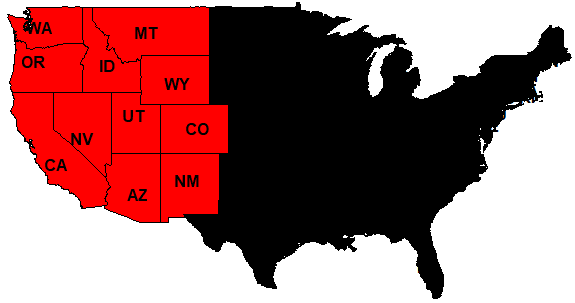
\includegraphics[width=1\textwidth]{WesternStatesNoTitleCropped.png} %
\caption{\label{fig:Map11States}Map of 11-state study area.} % The text after \label{} is what shows up as the caption. Inside the brackets for \label{} is just for linking figures to text and is analogous to the AuthorYear in citations. 
\end{figure} % end figure float

%%%%%%%%% Overview Maps %%%%%%%%%%%%

\subsubsection*{All PM2.5 Monitor Locations}
\begin{figure} 
\centering 
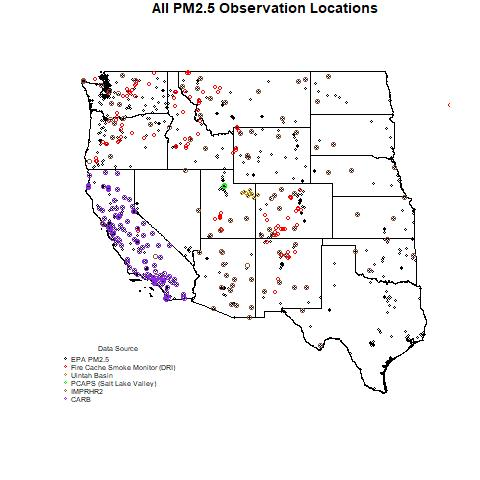
\includegraphics[width=0.77\textwidth]{Code_Outputs/MapPM25_All_Sitesplot_year0.jpg} 
\caption{\label{fig:MapPM25Loc0}Map of locations of PM2.5 observations for entire study period, 2008 to 2014.} 
\end{figure} 
 

\begin{figure} 
\centering 
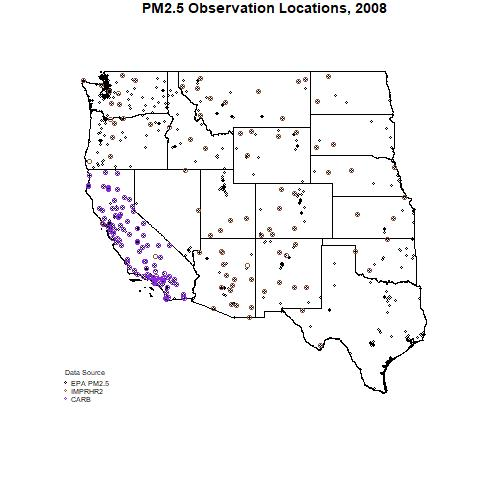
\includegraphics[width=0.77\textwidth]{Code_Outputs/MapPM25_All_Sitesplot_year2008.jpg} 
\caption{\label{fig:MapPM25Loc2008}Map of locations of PM2.5 observations during 2008.} 
\end{figure} 
 

\begin{figure} 
\centering 
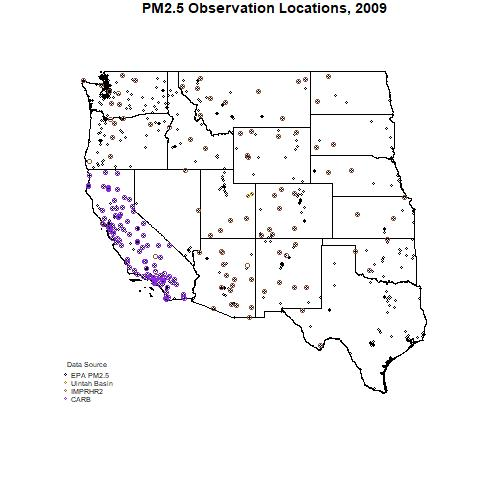
\includegraphics[width=0.77\textwidth]{Code_Outputs/MapPM25_All_Sitesplot_year2009.jpg} 
\caption{\label{fig:MapPM25Loc2009}Map of locations of PM2.5 observations during 2009.} 
\end{figure} 
 

\begin{figure} 
\centering 
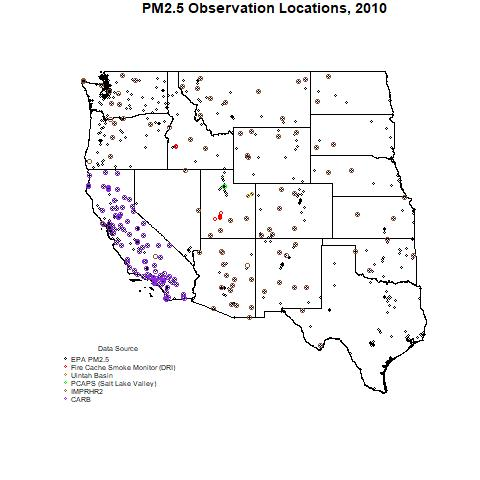
\includegraphics[width=0.77\textwidth]{Code_Outputs/MapPM25_All_Sitesplot_year2010.jpg} 
\caption{\label{fig:MapPM25Loc2010}Map of locations of PM2.5 observations during 2010.} 
\end{figure} 
 

\begin{figure} 
\centering 
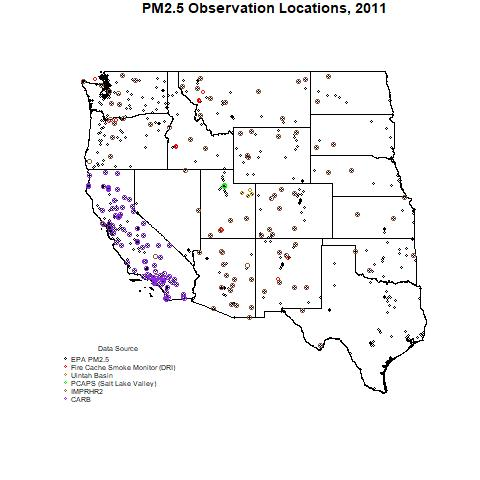
\includegraphics[width=0.77\textwidth]{Code_Outputs/MapPM25_All_Sitesplot_year2011.jpg} 
\caption{\label{fig:MapPM25Loc2011}Map of locations of PM2.5 observations during 2011.} 
\end{figure} 
 

\begin{figure} 
\centering 
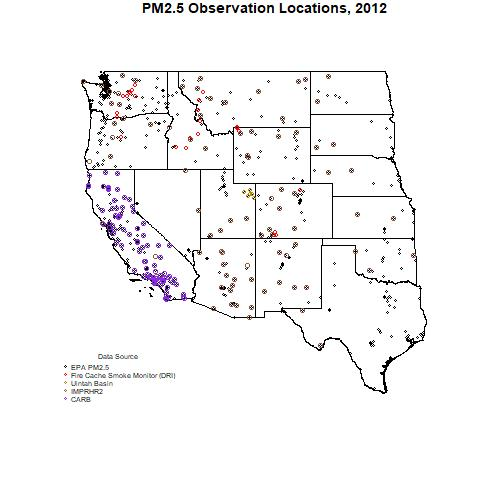
\includegraphics[width=0.77\textwidth]{Code_Outputs/MapPM25_All_Sitesplot_year2012.jpg} 
\caption{\label{fig:MapPM25Loc2012}Map of locations of PM2.5 observations during 2012.} 
\end{figure} 
 

\begin{figure} 
\centering 
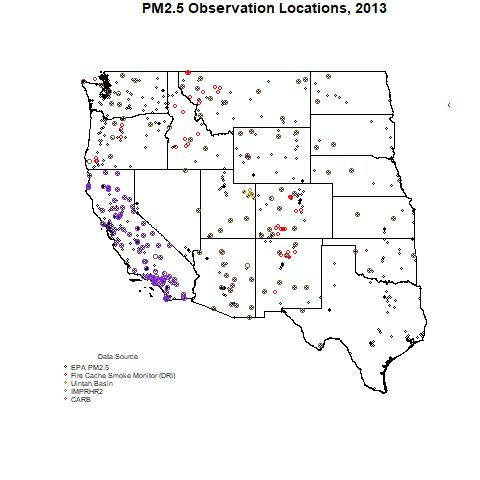
\includegraphics[width=0.77\textwidth]{Code_Outputs/MapPM25_All_Sitesplot_year2013.jpg} 
\caption{\label{fig:MapPM25Loc2013}Map of locations of PM2.5 observations during 2013.} 
\end{figure} 
 

\begin{figure} 
\centering 
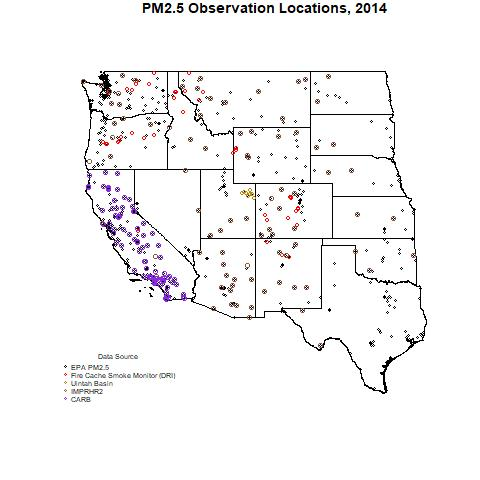
\includegraphics[width=0.77\textwidth]{Code_Outputs/MapPM25_All_Sitesplot_year2014.jpg} 
\caption{\label{fig:MapPM25Loc2014}Map of locations of PM2.5 observations during 2014.} 
\end{figure} 
 
 % created from R code, not to be edited directly

%%%%%%%%% PM2.5 Data Sources %%%%%%%%%%%%%%%%%%

\subsection{PM2.5 Monitor data from US EPA AQS Air Data Query Tool}

\subsubsection*{Data Source}

\begin{itemize}[nolistsep]
\item \textbf{Contact}

Can email the Air Quality Analysis Group (U.S. EPA Office of Air Quality Planning and Standards) on their website at \url{https://www.epa.gov/outdoor-air-quality-data/forms/contact-us-about-outdoor-air-quality-data}


\item \textbf{Citation/Link}

United States Environmental Protection Agency. \textit{Pre-Generated Data Files: Daily Summary Files, PM2.5 FRM/FEM Mass (88101) and PM2.5 non FRM/FEM Mass (88502), 2008-2014}. \url{https://aqs.epa.gov/aqsweb/airdata/download_files.html#Daily} 
\item \textbf{Data (local)}
\item \textbf{Geographic Extent}
\item \textbf{Temporal Extent}
2008 through 2014
\item \textbf{Acknowledgment}
\end{itemize}

\subsubsection*{Brief Description}

We will download PM\textsubscript{2.5} data from both the US EPA AQS Air Data Query Tool \citep{EPAAirData2017} and the IMPROVE monitors that capture air quality information in 
more rural areas \citep{EPANPM25IMPROVE2017} for the 11-state region (Figure \ref{fig:Map11States}) including any of the following parameter codes: 88101, 88500, 88502, 81104 \citep{EPANPM25Memo2017,EPANPM25Parameters2017,EPANAllParameters2017}. %In 2014, there were approximately 1600 PM\textsubscript{2.5} monitors (Figure \ref{fig:MapLocations}). For the 7-year study period, we anticipate approximately 1.4 million monitor-days. 

\subsubsection*{Notes}

\subsubsection*{File Format}

\subsubsection*{Data Filtering and Processing}

\subsubsection*{Final Variable(s)}

\subsubsection*{Methods}

\begin{enumerate}
\item 
\item
\end{enumerate}

\subsubsection*{Quality Control}

\subsubsection*{Script Names}

\begin{enumerate}
\item 
\end{enumerate}

\subsubsection*{Data File Names}

\begin{enumerate}
\item daily\_88101\_2008.csv
\item daily\_88101\_2009.csv
\item daily\_88101\_2010.csv
\item daily\_88101\_2011.csv
\item daily\_88101\_2012.csv
\item daily\_88101\_2013.csv
\item daily\_88101\_2014.csv
\item daily\_88502\_2008.csv
\item daily\_88502\_2009.csv
\item daily\_88502\_2010.csv
\item daily\_88502\_2011.csv
\item daily\_88502\_2012.csv
\item daily\_88502\_2013.csv
\item daily\_88502\_2014.csv
\end{enumerate} 

\begin{figure}[H] % start figure float, this method seems to have fewer options for location specifier, H, t, c, and b should work
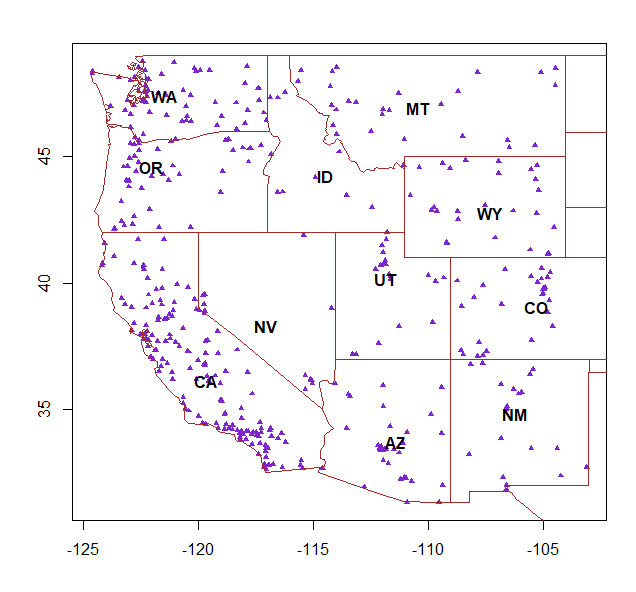
\includegraphics[width=1\textwidth]{m88101and88502notitlenorlabels.PNG} %
\caption{\label{fig:MapLocations}Map of 88101 and 88502 PM\textsubscript{2.5} Monitors.} % The text after \label{} is what shows up as the caption. Inside the brackets for \label{} is just for linking figures to text and is analogous to the AuthorYear in citations. 
\end{figure} % end figure float
 


\subsection*{EPA PM2.5 Plots}
\begin{figure} 
\centering 
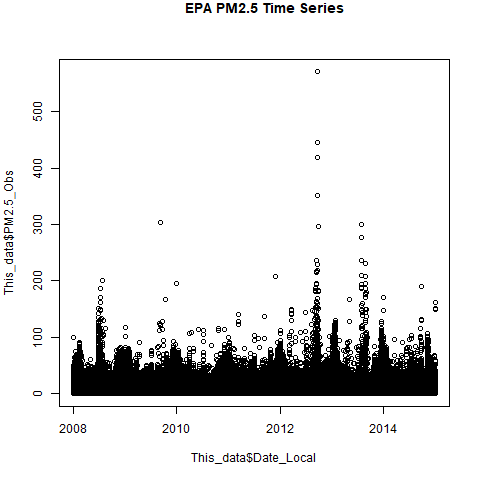
\includegraphics[width=0.77\textwidth]{Code_Outputs/EPA_PM25_time_series.png} 
\caption{\label{fig:EPA_PM25TS}EPA PM2.5 time series.} 
\end{figure} 
 
 % created from R code, not to be edited in Overleaf

%\subsection{PM2.5 Monitor data from IMPROVE network}

\subsubsection*{Data Source}

\begin{itemize}[nolistsep]
\item \textbf{Contact}
\item \textbf{Citation/Link}
\item \textbf{Data (local)}
\item \textbf{Geographic Extent}
\item \textbf{Temporal Extent}
\item \textbf{Acknowledgment}
\end{itemize}

\subsubsection*{Brief Description}

We will download PM\textsubscript{2.5} data from both the US EPA AQS Air Data Query Tool \citep{EPAAirData2017} and the IMPROVE monitors that capture air quality information in 
more rural areas \citep{EPANPM25IMPROVE2017} for the 11-state region (Figure \ref{fig:Map11States}) including any of the following parameter codes: 88101, 88500, 88502, 81104 \citep{EPANPM25Memo2017,EPANPM25Parameters2017,EPANAllParameters2017}. %In 2014, there were approximately 1600 PM\textsubscript{2.5} monitors (Figure \ref{fig:MapLocations}). For the 7-year study period, we anticipate approximately 1.4 million monitor-days. 

\subsubsection*{Notes}

\subsubsection*{File Format}

\subsubsection*{Data Filtering and Processing}

\subsubsection*{Final Variable(s)}

\subsubsection*{Methods}

\begin{enumerate}
\item 
\item
\end{enumerate}

\subsubsection*{Quality Control}

\subsubsection*{Script Names}

\begin{enumerate}
\item 
\end{enumerate}

\subsubsection*{Data File Names}

\begin{enumerate}
\item 
\end{enumerate} % IMPROVE data is in the Federal Land Manager Environmental Database

%\include{CalNex2010PM25Data}

\subsubsection{\texorpdfstring{PM\textsubscript{2.5}}{} data from the Federal Land Manager Environmental Database} \label{IMPROVE}

\subsubsection*{To Do}
\begin{enumerate}
\item Check again to see if the 2018 data is available (as of February 2019, it was not available)
\end{enumerate}

\subsubsection*{Data Source}

\begin{itemize}[nolistsep]
% Tom Moore directed us to the website
\item \textbf{Contact} Bret Schichtel
\item \textbf{Citation/Link} \url{http://views.cira.colostate.edu/fed/DataWizard/Default.aspx}
\item \textbf{Download Date} March 15, 2018%February 13, 2018 %February 2, 2018
\item \textbf{Data (local)} PM\textsubscript{2.5} data from the Federal Land Manager Environmental Database
\item \textbf{Geographic Extent} Nationwide
\item \textbf{Temporal Extent} January 1, 2008 - Decemer 31, 2017 %January 1, 2008 - December 31, 2014
\item \textbf{Acknowledgment} - need to fill in
\end{itemize}

%UNCOMMENT \subsubsection*{Brief Description}

%UNCOMMENT We will download PM\textsubscript{2.5} data from both the US EPA AQS Air Data Query Tool \citep{EPAAirData2017} and the IMPROVE monitors that capture air quality information in 
%UNCOMMENT more rural areas \citep{EPANPM25IMPROVE2017} for the 11-state region (Figure \ref{fig:Map11States}) including any of the following parameter codes: 88101, 88500, 88502, 81104 \citep{EPANPM25Memo2017,EPANPM25Parameters2017,EPANAllParameters2017}. %In 2014, there were approximately 1600 PM\textsubscript{2.5} monitors (Figure \ref{fig:MapLocations}). For the 7-year study period, we anticipate approximately 1.4 million monitor-days. 

We downloaded IMPROVE PM\textsubscript{2.5} data from the Federal Land Manager Environmental Database maintained by CIRA and Colorado State University. The IMPROVE monitors capture air quality information in more rural areas \citep{EPANPM25IMPROVE2017}. We are including any of the following parameter codes: 88101, 88500, 88502, 81104 \citep{EPANPM25Memo2017,EPANPM25Parameters2017,EPANAllParameters2017}.

The data does not come with datum information. When processing the data, the datum is input as WGS84 per an email from Bret Schichtel on October 22, 2018.

A few sites only had only two decimal places for latitude and/or longitude. I contacted Bret Schichtel (bret.schichtel@colostate.edu), who put me in contact with Scott Copeland (scott.copeland@colostate.edu) and Anthony Prenni (anthony\_prenni@nps.gov). Scott Copeland sent Site\_Meta\_Master\_10\_2018.csv, a master file of the IMPROVE sites and Anthony Prenni referred me to the ``Current Site List'' at \url{http://vista.cira.colostate.edu/Improve/improve-data/}. The Current Site List seems to have the most decimal places for location information, but does not have all sites. This file is used first and then locations are filled in from Site\_Meta\_Master\_10\_2018.csv. Latitude and Longitude data from the main data files are ignored. See process\_PM25\_IMPROVE\_data\_source\_functions.R.
\bigskip

%\noindent Downloading IMPROVE Aerosol, RHR III (DRAFT-Preliminary...) data: 
\noindent Downloading IMPROVE Aerosol, RHR II (New Equation) data (one parameter at at time):
\begin{enumerate}
\item Reports: Raw data
\item Datasets:``IMPROVE Aerosol, RHR II (New Equation)''
\item Sites: select all
\item Parameters: 
  \begin{enumerate}
  \item Mass, PM2.5 (Fine): Code MF, Type PM2.5, Units ug/m\^3 LC AQS ID 88101
  \item Mass, PM2.5 Reconstructed (Fine): Code RCFM, Type PM2.5 Units ug/m\^3 LC, AQS ID 88401
  \end{enumerate}
\item Select Dates: By Years and Months: 2008-2017; select all months
\item Aggregations: Non-aggregated
\item Fields: Select All
\item When 2008-2014 data was downloaded: Options: Text File; Generate one file containing all the data; Comma delimited, Standard (``wide'' format); Data \& Metadata, Display Column Headers, Don't Display Section Titles, String Quotes: Double Quotes, Missing Values (blank); Date Format: 3/14/2002; Display Results: In a separate browser window; Show Report Log
\item When 2008-2017 data was downloaded: Options: Text File; Generate one file containing all the data; Comma delimited, Standard (``wide'' format); Data \& Metadata, %Display Column Headers, Don't Display Section Titles, 
String Quotes: Double Quotes, Missing Values (blank); Date Format: 3/14/2002; Display Results: In a separate browser window; %Show Report Log

\item Submit
\end{enumerate}

Repeat the downloading steps above, except replace step \#2 with these Datasets and parameters:
\begin{enumerate}
\item IMPROVE Aerosol, RHR III (DRAFT - Preliminary Most Impaired Days dataset) 
	\begin{enumerate}
	\item Mass, PM2.5 (Fine) is listed twice %for the 2008-2014 data these turned out to be the same data%, download one at a time - referred to as `first param' and `second param' in file names - these turned out to be the same data
	\end{enumerate}
\end{enumerate}

After downloading data, save each file as *\_top\_removed.csv and remove all rows above the main section of data (approximately 270 rows). 


%UNCOMMENT \subsubsection*{Notes}

%UNCOMMENT Data sets in this database that don't work for this project:
%UNCOMMENT \begin{enumerate}
%UNCOMMENT \item ``SEARCH FRM" is only available 1998-2005
%UNCOMMENT \item ``SEARCH Best Estimate'' is only available 1998-2005
%UNCOMMENT \end{enumerate}

%UNCOMMENT 2018-05-29; \url{http://views.cira.colostate.edu/fed/User/Feedback.aspx}
%UNCOMMENT ``Hello Federal Land Manager Environmental Database,

%UNCOMMENT I have downloaded several files from http://views.cira.colostate.edu/fed/DataWizard/Default.aspx for my research. How can I determine which datum (e.g., WGS84, NAD83, etc.) is associated with the latitude and longitude data in those files?

%UNCOMMENT Thank you, 
%UNCOMMENT Melissa May Maestas, PhD
%UNCOMMENT Research Associate (Post-Doctoral)
%UNCOMMENT University of Colorado Boulder
%UNCOMMENT e: Melissa.Maestas@Colorado.edu''

%UNCOMMENT Auto-reply:
%UNCOMMENT ``Thanks for your feedback!
%UNCOMMENT Your message has been sent to the project team and will be directed to the appropriate person. At least one team member will personally read your message. For those questions or comments that require a direct response, we will try to respond as quickly as possible. Reported errors will be logged immediately and addressed according to severity, ease of identification, and ease of resolution. Comments and suggestions regarding features, improvements, and content will be logged, prioritized, and addressed in upcoming development cycles.
%UNCOMMENT We greatly appreciate your comments and questions. We are striving to provide you with quality data products and the best web site experience possible, and your comments are greatly valued as we seek to improve and expand our web site. Your participation is a key component in the success and usefulness of the website. ``

\subsubsection*{File Formats} 
csv

%UNCOMMENT \subsubsection*{Data Filtering and Processing}



%UNCOMMENT \subsubsection*{Final Variable(s)}

%UNCOMMENT \subsubsection*{Methods}

%UNCOMMENT \begin{enumerate}
%UNCOMMENT \item 
%UNCOMMENT \item
%UNCOMMENT \end{enumerate}

%UNCOMMENT \subsubsection*{Quality Control}

%UNCOMMENT \subsubsection*{Script Names}

%UNCOMMENT \begin{enumerate}
%UNCOMMENT \item 
%UNCOMMENT \end{enumerate}

\subsubsection*{Original Data File Names}

\begin{enumerate}[noitemsep]
\item Federal\_Land\_Manager\_IMPROVE\_RHR\_II\_88101\_201922513514530P22rMs.csv % 2008-2014 data
\item Federal\_Land\_Manager\_IMPROVE\_RHR\_II\_88401\_20192251356232212121t.csv  % 2008-2014 data
\item  Federal\_Land\_Manager\_RHR\_III\_88101\_first\_param\_2019225135946946xJ0L22.csv  % 2008-2014 data

%\item Federal\_Land\_Manager\_IMPROVE\_RHR\_II\_88101\_20183151757452922Mvw0s.csv % 2008-2014 data
%\item Federal\_Land\_Manager\_IMPROVE\_RHR\_II\_88401\_20185113533660420xLwJ.csv  % 2008-2014 data
%\item  Federal\_Land\_Manager\_RHR\_III\_88101\_first\_param\_201851152033932P22My0.csv  % 2008-2014 data

\end{enumerate}

%UNCOMMENT \subsubsection*{Processed/Cleaned Data File Names}

%UNCOMMENT \begin{enumerate}
%\item Federal\_Land\_Manager\_IMPROVE\_RHR\_II\_2018315132109KL0L2K\_top\_removed.csv (removed header information that explains codes, etc.)
%UNCOMMENT \item Federal\_Land\_Manager\_IMPROVE\_RHR\_II\_88101\_20183151757452922Mvw0s\_top\_removed.csv
%UNCOMMENT \item Federal\_Land\_Manager\_IMPROVE\_RHR\_II\_88401\_20185113533660420xLwJ\_top\_removed.csv
%UNCOMMENT \item Federal\_Land\_Manager\_RHR\_III\_88101\_first\_param\_201851152033932P22My0\_top\_removed.csv
%UNCOMMENT \item Federal\_Land\_Manager\_RHR\_III\_second\_param\_2018511545575622rOMxr\_top\_removed.csv
%UNCOMMENT \end{enumerate}
 

%
\subsection{IMPRHR2 Plots}
\begin{figure} 
\centering 
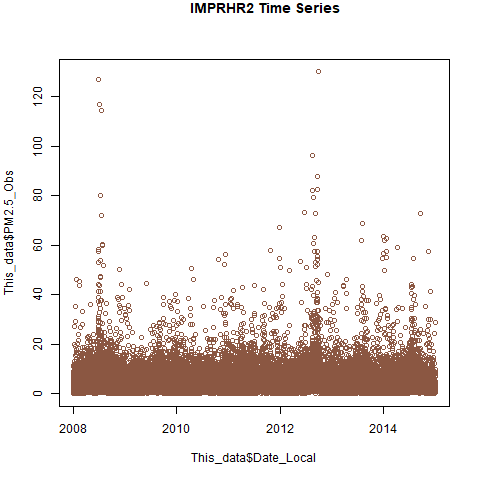
\includegraphics[width=0.77\textwidth]{Code_Outputs/IMPRHR2_time_series.png} 
\caption{\label{fig:IMPRHR2TS}IMPRHR2 time series.} 
\end{figure} 
 
 % created from R code, not to be edited in Overleaf
%
\subsection{IMPRHR2 MF II Plots}
\begin{figure} 
\centering 
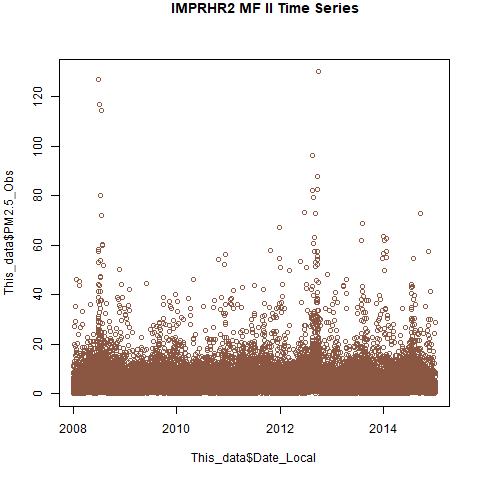
\includegraphics[width=0.77\textwidth]{Code_Outputs/IMPRHR2MFII_time_series.png} 
\caption{\label{fig:IMPRHR2MFIITS}IMPRHR2 MF II time series.} 
\end{figure} 
 
 % created from R code, not to be edited directly

%
\subsection{IMPRHR2 RCFM Plots}
\begin{figure} 
\centering 
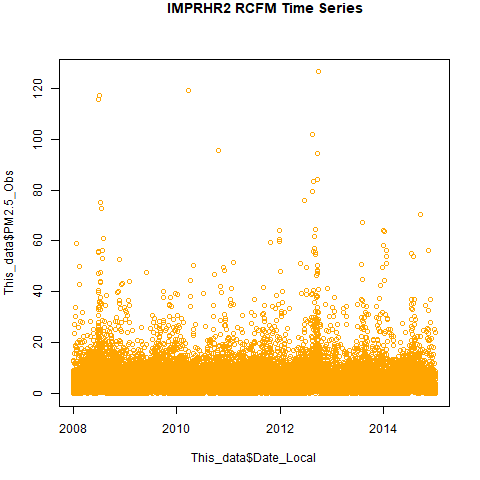
\includegraphics[width=0.77\textwidth]{Code_Outputs/IMPRHR2RCFM_time_series.png} 
\caption{\label{fig:IMPRHR2RCFMTS}IMPRHR2 RCFM time series.} 
\end{figure} 
 
 % created from R code, not to be edited directly

%
\subsection{IMPRHR3 MF III1 Plots}
\begin{figure} 
\centering 
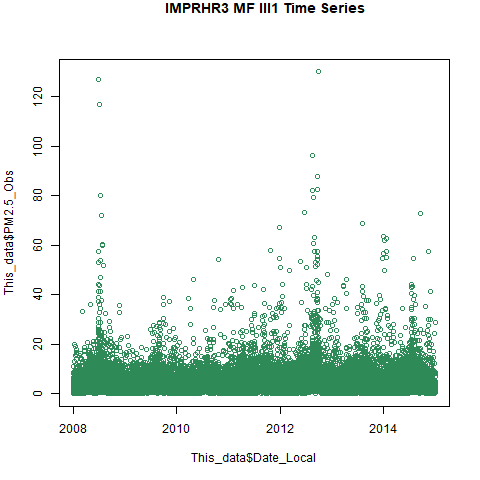
\includegraphics[width=0.77\textwidth]{Code_Outputs/IMPRHR3MFIII1_time_series.png} 
\caption{\label{fig:IMPRHR3MFIII1TS}IMPRHR3 MF III1 time series.} 
\end{figure} 
 
 % created from R code, not to be edited directly

%
\subsection{IMPRHR3 MF III2 Plots}
\begin{figure} 
\centering 
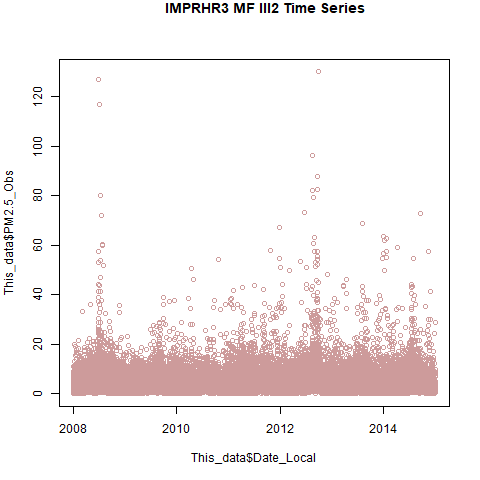
\includegraphics[width=0.77\textwidth]{Code_Outputs/IMPRHR3MFIII2_time_series.png} 
\caption{\label{fig:IMPRHR3MFIII2TS}IMPRHR3 MF III2 time series.} 
\end{figure} 
 
 % created from R code, not to be edited directly

%
\subsection{IMPRHR2 RCFM Plots}
\begin{figure} 
\centering 
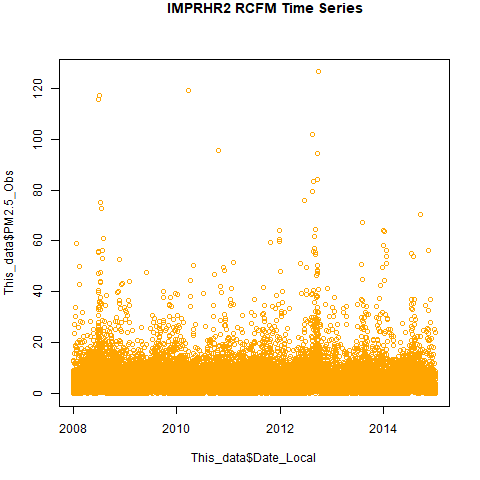
\includegraphics[width=0.77\textwidth]{Code_Outputs/IMPRHR2RCFM_time_series.png} 
\caption{\label{fig:IMPRHR2RCFMTS}IMPRHR2 RCFM time series.} 
\end{figure} 
 
 % created from R code, not to be edited directly



%\include{Rgenerated_ImagesFedLndMng} % created from R code, not to be edited in Overleaf

\subsection{\texorpdfstring{PM\textsubscript{2.5}}{} data from the Fire Cache Smoke Monitor Archive}

\subsubsection*{Data Source}

\begin{itemize}[nolistsep]
\item \textbf{Contact} Amber Ortega directed us to the website and Scott Landis suggested that a good person to contact about the page would be Mike Broughton from the US Forest Service (\url{michaelbroughton@fs.fed.us})
\item \textbf{Citation/Link} \url{https://wrcc.dri.edu/cgi-bin/smoke.pl}
\item \textbf{Data (local)} PM\textsubscript{2.5} data from the Fire Cache Smoke Monitor Archive
\item \textbf{Geographic Extent} 
\item \textbf{Temporal Extent} 
\item \textbf{Acknowledgment} 
\end{itemize}

\subsubsection*{Brief Description}

\subsubsection*{Notes}

Files Fire\_Cache\_Smoke\_DRI\_Smoke\_E-BAM\_231.csv and Fire\_Cache\_Smoke\_DRI\_Smoke\_E-BAM\_866.csv were deleted because it only had data across 3 days, but none of them met the basic requirements to be put into the final data (e.g., not enough observations or negative concentrations).

Fire\_Cache\_Smoke\_DRI\_Smoke\_E\_BAM\_65.csv was also deleted because it only had 5 data points across 2 days, and we are requiring at least 18 hourly data points within a day to be put into the final data.

\subsubsection*{File Formats} 
.dat

\subsubsection*{Data Filtering and Processing}

\subsubsection*{Final Variable(s)}

\subsubsection*{Methods}

\begin{enumerate}
\item 
\item
\end{enumerate}

\subsubsection*{Quality Control}

\subsubsection*{Script Names}

\begin{enumerate}
\item 
\end{enumerate}

\subsubsection*{Original Data File Names}

\begin{enumerate}
\item Fire\_Cache\_Smoke\_DRI\_FWS\_Smoke\_N1.csv
\item Fire\_Cache\_Smoke\_DRI\_Smoke\_N11.csv
\item Fire\_Cache\_Smoke\_DRI\_Smoke\_N13.csv
\item Fire\_Cache\_Smoke\_DRI\_Smoke\_N15.csv
\item Fire\_Cache\_Smoke\_DRI\_Smoke\_N16.csv
\item Fire\_Cache\_Smoke\_DRI\_Smoke\_N17.csv
\item Fire\_Cache\_Smoke\_DRI\_Smoke\_N19.csv
\item Fire\_Cache\_Smoke\_DRI\_Smoke\_N20.csv
\item Fire\_Cache\_Smoke\_DRI\_Smoke\_N21.csv
\item Fire\_Cache\_Smoke\_DRI\_Smoke\_N22.csv
\item Fire\_Cache\_Smoke\_DRI\_Smoke\_N23.csv
\item Fire\_Cache\_Smoke\_DRI\_Smoke\_N24.csv
\item Fire\_Cache\_Smoke\_DRI\_Smoke\_N25.csv
\item Fire\_Cache\_Smoke\_DRI\_Smoke\_N65.csv
\item Fire\_Cache\_Smoke\_DRI\_Smoke\_N66.csv
\item Fire\_Cache\_Smoke\_DRI\_Smoke\_N67.csv
\item Fire\_Cache\_Smoke\_DRI\_Smoke\_N68.csv
\item Fire\_Cache\_Smoke\_DRI\_Smoke\_N69.csv
\item Fire\_Cache\_Smoke\_DRI\_Smoke\_N84.csv
\item Fire\_Cache\_Smoke\_DRI\_Smoke\_N215.csv
\item Fire\_Cache\_Smoke\_DRI\_Smoke\_N216.csv
\item Fire\_Cache\_Smoke\_DRI\_Smoke\_N217.csv
\item Fire\_Cache\_Smoke\_DRI\_Smoke\_E\_BAM\_52.csv
\item Fire\_Cache\_Smoke\_DRI\_Smoke\_E\_BAM\_65.csv
\item Fire\_Cache\_Smoke\_DRI\_Smoke\_E-BAM\_840.csv
\item Fire\_Cache\_Smoke\_DRI\_Smoke\_E-BAM\_925.csv
\item Fire\_Cache\_Smoke\_DRI\_Smoke\_USFS\_R1-39.csv
\item Fire\_Cache\_Smoke\_DRI\_Smoke\_USFS\_R1-52.csv
\item Fire\_Cache\_Smoke\_DRI\_Smoke\_USFS\_R1-53.csv
\item Fire\_Cache\_Smoke\_DRI\_Smoke\_USFS\_R1-306.csv
\item Fire\_Cache\_Smoke\_DRI\_Smoke\_USFS\_R1-307.csv
\item Fire\_Cache\_Smoke\_DRI\_Smoke\_USFS\_R2-78.csv
\item Fire\_Cache\_Smoke\_DRI\_Smoke\_USFS\_R2-264.csv
\item Fire\_Cache\_Smoke\_DRI\_Smoke\_USFS\_R2-265.csv
\item Fire\_Cache\_Smoke\_DRI\_Smoke\_USFS\_R3-28.csv
\item Fire\_Cache\_Smoke\_DRI\_Smoke\_USFS\_R3-86.csv
\item Fire\_Cache\_Smoke\_DRI\_Smoke\_USFS\_R5-39.csv
\item Fire\_Cache\_Smoke\_DRI\_Smoke\_USFS\_R5-49.csv
\item Fire\_Cache\_Smoke\_DRI\_Smoke\_USFS\_R9-15.csv
\item Fire\_Cache\_Smoke\_DRI\_Smoke\_USFS\_R9-16.csv
\item Fire\_Cache\_Smoke\_DRI\_Smoke\_USFS\_R9-17.csv
\item Fire\_Cache\_Smoke\_DRI\_Smoke\_USFS\_R9-60.csv

\end{enumerate}

\subsubsection*{Processed/Cleaned Data File Names}

\begin{enumerate}
\item 
\item
\end{enumerate}

\subsection*{Download instructions}
\begin{enumerate}
\item \url{https://wrcc.dri.edu/cgi-bin/smoke.pl}
\item Hover over the appropriate drop-down menu and click on the monitor you want to download e.g., “Cache Monitors” then “Smoke \#11”
\item On the left-side menu, click on “Data Details”
\item Set the starting date: January 1, 2008 (or as far back as it goes if it doesn’t go back to 2008)
\item Set the ending date: December 31, 2014 (or the last date possible if it ends before 2014)
\item Elements (ignore - default is to include all elements)
\item Options
\item Excel (.xls) (It had html code in the file if I chose other options.)
\item Data Source: Original
\item Represent missing data as: -9999. 
\item Include data flags: Yes
\item Date format: MM/DD/YYYY hh:mm
\item Time format: LST 0-23
\item Table Header: Column header short descriptions
\item Field Delimiter: comma (,)
\item Select the Units: Metric
\item Leave Sub interval windows set to: January 01, December 31, Hours: 00 and 24
\item Submit Info
\item Open in excel
\item Save as: Fire\_Cache\_Smoke\_DRI\_*.csv Where * is the monitor name with spaces replaced with underscore and \# symbols replaced with the letter N, e.g., the file name for monitor “Smoke \#11” is “Fire\_Cache\_Smoke\_DRI\_Smoke\_N11.csv”
\item Upload file to S3 bucket: \url{https://732215511434.signin.aws.amazon.com/console}
\item Click on S3
\item Earthlab-reid-group
\item Fire\_Cache\_Smoke\_DRI (folder)
\item Check the following:
\item The name of the monitor is in cell A1
\item The header is spread across rows 2-4
\item There are 34 columns of data (goes through columns “AH” in excel)
\item Concentration in the 11th (“K”) columns
\item List the file names in the overleaf documentation (PM25\_Fire\_Cache\_Smoke\_Monitor\_Archive.tex)







\end{enumerate}
 % UNCOMMENT


\subsection*{Fire Cache Smoke Monitor (DRI) Plots}
\begin{figure} 
\centering 
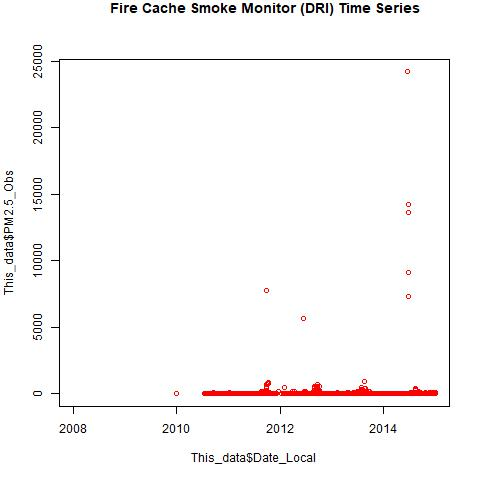
\includegraphics[width=0.77\textwidth]{Code_Outputs/FireCacheDRI_time_series.jpg} 
\caption{\label{fig:FireCacheDRITS}Fire Cache Smoke Monitor (DRI) time series.} 
\end{figure} 
 
 % created from R code, not to be edited in Overleaf

\subsubsection{\texorpdfstring{PM\textsubscript{2.5}}{} data from the California State Air Quality and Meteorological Information System (AQMIS)}

\subsubsection*{To Do}
\begin{enumerate}
\item Check for availability of 2015-2018 data
\end{enumerate}

\subsubsection*{Data Source}

\begin{itemize}[nolistsep]
\item \textbf{Contact} Denise Odenwalder, Denise.Odenwalder@arb.ca.gov
\item \textbf{Citation/Link} To AQMIS: \url{https://www.arb.ca.gov/aqmis2/aqmis2.php}
\item \textbf{Data (local)} 
\item \textbf{Geographic Extent} Whole state of California, wherever there are monitors
\item \textbf{Temporal Extent} 2008-2014, daily averages
\item \textbf{Acknowledgment} California Air Resources Board was very helpful in gathering and sending us this data.
\end{itemize}

\subsubsection*{Brief Description}

\begin{itemize}
\item PM2.5 measurements at all monitoring stations in CA
\item Some entries are 24-hour measurements while others are the average of hourly measurements
\item One entry per 3 days
\end{itemize}

\subsubsection*{Notes}

Reached out to aqmis@arb.ca.gov after determining that there was data being collected in CA that is not published on the EPA AQS website. They emailed us within a week, with a file of the data we requested. 

\subsubsection*{File Formats} 
xlsx spreadsheet

\subsubsection*{Data Filtering and Processing}

\subsubsection*{Final Variable(s)}

\subsubsection*{Methods}

\begin{enumerate}
\item 
\item
\end{enumerate}

\subsubsection*{Quality Control}

\subsubsection*{Script Names}

\begin{enumerate}
\item 
\end{enumerate}

\subsubsection*{Original Data File Names}

\begin{enumerate}
\item 
\item 
\end{enumerate}

\subsubsection*{Processed/Cleaned Data File Names}

\begin{enumerate}
\item 
\item 
\end{enumerate}



\subsection*{CARB Plots}
\begin{figure} 
\centering 
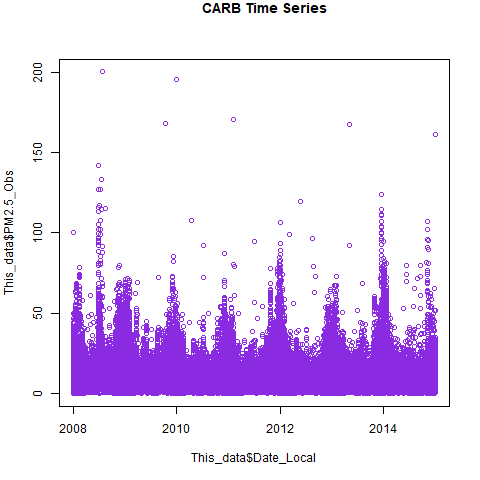
\includegraphics[width=0.77\textwidth]{Code_Outputs/CARB_time_series.png} 
\caption{\label{fig:CARBTS}CARB time series.} 
\end{figure} 
 
 % created from R code, not to be edited directly

\subsubsection{\texorpdfstring{PM\textsubscript{2.5}}{} Monitor data from Uintah Basin}

\subsubsection*{To Do}
\begin{enumerate}
\item Check to see if there is any more recent data available
\end{enumerate}

\subsubsection*{Data Source}

\begin{itemize}[nolistsep]
\item \textbf{Contact} Seth Lyman 
\item \textbf{Citation/Link} seth.lyman@usu.edu
\item \textbf{Data (local)} PM\textsubscript{2.5} measurements from 10 sites in Uintah Basin, Utah
\item \textbf{Geographic Extent} Uintah Basin, Utah
\item \textbf{Temporal Extent} October 2009 - March 2017
\item \textbf{Acknowledgment} PM\textsubscript{2.5} data from the Uintah Basin were provided by Seth Lyman at Utah State University.
\end{itemize}

\subsubsection*{Brief Description}

PM\textsubscript{2.5} data were provided by Seth Lyman at Utah State University via email on January 16, 2018. The .xlsx file has PM\textsubscript{2.5} data from 10 stations during 2009-2017. The .png file has the longitude and latitude of each site. 

\subsubsection*{Notes}
Additional information from Seth's email: \newline
``I’ve attached most of the PM2.5 observations that have ever been collected in the Uintah Basin.  What are in the Excel file are 24-hr average data.  Data from Roosevelt, Vernal, Ouray, Red Wash, Myton, and Rangely are from the EPA AQS database. \newline Data from Horsepool are from a BAM 1020 monitor that we operate every winter.  Data in Ft. Duchesne and Randlett are 24-hr filter samples that were analyzed gravimetrically.  Data from Rabbit Mountain are from a BAM 1020, and data through mid-2013 are in the AQS database. \newline \newline
\noindent I have hourly data from Horsepool and Rabbit Mountain if you’d rather have that. \newline \newline
\noindent Site locations are given in the list of monitoring stations for the Basin below.'' \newline

The .png file is easier to read in some programs than others, e.g., it looks fine in ``Paint,'' but not ``Photos.''

\subsubsection*{File Formats} 
Excel and png

\subsubsection*{Data Filtering and Processing}
FinalPM2.5\_multiyear\_thruwint2017\_sheet1.csv is the first sheet of FinalPM2.5\_multiyear\_thruwint2017.xlsx converted to .csv, and the second row of the header was merged into the first (24hr avg PM2.5).

FinalPM2.5\_multiyear\_thruwint2017\_GISsheet.csv is the third sheet of FinalPM2.5\_multiyear\_thruwint2017.xlsx converted to .csv and gives the latitude and longitude of each site. This sheet originally did not have location information from the Rangely site, so this was filled in by hand with the numbers form UintahBasinSiteLocations.png.


\subsubsection*{Final Variable(s)}

\subsubsection*{Methods}

\begin{enumerate}
\item 
\item
\end{enumerate}

\subsubsection*{Quality Control}

\subsubsection*{Script Names}

\begin{enumerate}
\item 
\end{enumerate}

\subsubsection*{Original Data File Names}

\begin{enumerate}
\item FinalPM2.5\_multiyear\_thruwint2017.xlsx
\item UintahBasinSiteLocations.png
\end{enumerate}

\subsubsection*{Processed/Cleaned Data File Names}

\begin{enumerate}
\item FinalPM2.5\_multiyear\_thruwint2017\_sheet1.csv%FinalPM2.5\_multiyear\_thruwint2017_sheet1.csv
\item UintahBasinSiteLocations.png
\end{enumerate} 

%
\subsection*{Uintah Basin Plots}
\begin{figure} 
\centering 
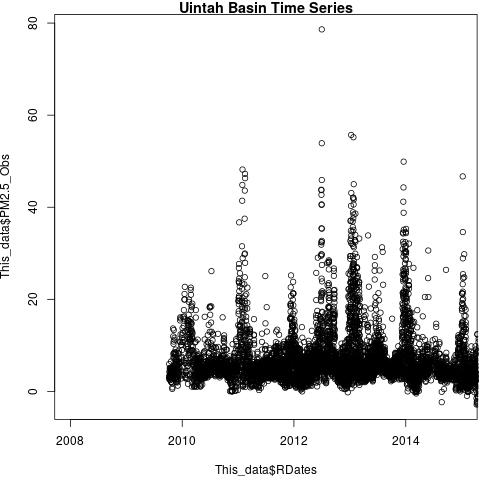
\includegraphics[width=0.77\textwidth]{Code_Outputs/UintahBasin_time_series.jpg} 
\caption{\label{fig:UintahBasinTS}Uintah Basin time series.} 
\end{figure} 
 
 % created from R code, not to be edited in Overleaf

\subsubsection{\texorpdfstring{PM\textsubscript{2.5}}{} data from PCAPS in the Salt Lake Valley}

\subsubsection*{Data Source}

\begin{itemize}[nolistsep]
\item \textbf{Contact} Dr. Geoff Silcox in Chemical Engineering at the University of Utah (\url{geoff@chemeng.utah.edu})
\item \textbf{Citation/Link} Publication: \url{https://www.sciencedirect.com/science/article/pii/S1352231011011204} \cite{Silcox_wintertime_2012} (Data was received from Dr. Silcox via email on February 6, 2018.)
\item \textbf{Data (local)} PM\textsubscript{2.5} data from the Persistent Cold Air Pool Study (PCAPS)
\item \textbf{Geographic Extent} Salt Lake Valley
\item \textbf{Temporal Extent} January - February, 2011
\item \textbf{Acknowledgment} Dr. Geoff Silcox
\end{itemize}

\subsubsection*{Brief Description}

\subsubsection*{Notes}

\subsubsection*{File Formats} 
.xlsx

\subsubsection*{Data Filtering and Processing}

PCAPS\_Site\_Locations.csv is the same data as Table 1 of final\_publication.pdf, and has the site locations and elevation.

\subsubsection*{Final Variable(s)}

\subsubsection*{Methods}

\begin{enumerate}
\item 
\item
\end{enumerate}

\subsubsection*{Quality Control}

\subsubsection*{Script Names}

\begin{enumerate}
\item 
\end{enumerate}

\subsubsection*{Original Data File Names}

\begin{enumerate}
\item final\_publication.pdf (Publication of paper)

\item MiniVol\_data.xlsx

\end{enumerate}

\subsubsection*{Processed/Cleaned Data File Names}

\begin{enumerate}
\item MiniVol\_data.csv
\item PCAPS\_Site\_Locations.csv
\end{enumerate}

%
\subsection{PCAPS (Salt Lake Valley) Plots}
\begin{figure} 
\centering 
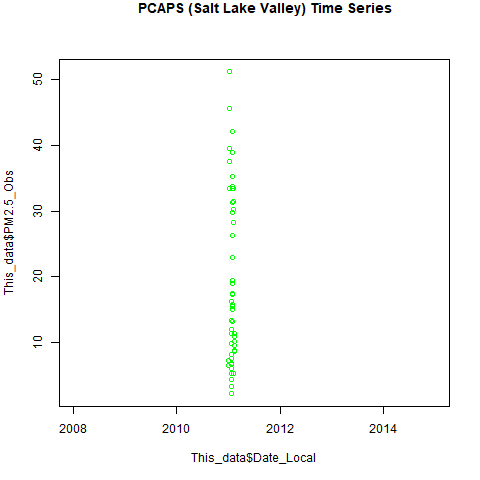
\includegraphics[width=0.77\textwidth]{Code_Outputs/PCAPS_time_series.png} 
\caption{\label{fig:PCAPSTS}PCAPS (Salt Lake Valley) time series.} 
\end{figure} 
 
 % created from R code, not to be edited in Overleaf 

%\subsection{Arizona Deparment of Environmental Quality (ADEQ)}

\subsubsection*{Data Source}

\begin{itemize}[nolistsep]
\item \textbf{Contact}  Phone: 602-771-7676; also email option on website
\item \textbf{Citation/Link} \url{http://azdeq.gov/node/2204}
\item \textbf{Data (local)} 
\item \textbf{Geographic Extent} 
\item \textbf{Temporal Extent} 
Only has data archived 2016 - 2017
\item \textbf{Acknowledgment} 
\end{itemize}

\subsubsection*{Brief Description}

\subsubsection*{Notes}

\subsubsection*{File Formats} 

\subsubsection*{Data Filtering and Processing}

\subsubsection*{Final Variable(s)}

\subsubsection*{Methods}

\begin{enumerate}
\item 
\item
\end{enumerate}

\subsubsection*{Quality Control}

\subsubsection*{Script Names}

\begin{enumerate}
\item 
\end{enumerate}

\subsubsection*{Original Data File Names}

\begin{enumerate}
\item 
\item 
\end{enumerate}

\subsubsection*{Processed/Cleaned Data File Names}

\begin{enumerate}
\item 
\item 
\end{enumerate}


%Not using this since NV DEQ emailed Ellen Considine that all the processed data (that they recommended using) is available through AQS (see email from May 29, 2018). %\subsection{Additional Air Quality Data from the Nevada Department of Environmental Quality}
\subsection{Nevada Department of Environmental Quality}

\subsubsection*{Data Source}

\begin{itemize}[nolistsep]
\item \textbf{Contact} 
\item \textbf{Citation/Link} \url{http://nvair.ndep.nv.gov/}
\item \textbf{Data (local)} 
\item \textbf{Geographic Extent} Ranchos Site (820 Lyell Way (Aspen Park Maintenance Yard), Gardnerville; GPS: +38.897557, -119.732507) \url{https://ndep.nv.gov/uploads/air-aqm-docs/2017-air-monitoring-network.pdf } (page 49)
\item \textbf{Temporal Extent} 2008-2009
\item \textbf{Acknowledgment} 
\end{itemize}

\subsubsection*{Brief Description}
Pm2.5 measures; daily average


\subsubsection*{Notes}

\subsubsection*{File Formats} 

\subsubsection*{Data Filtering and Processing}

\subsubsection*{Final Variable(s)}

\subsubsection*{Methods}

\begin{enumerate}
\item 
\item
\end{enumerate}

\subsubsection*{Quality Control}

\subsubsection*{Script Names}

\begin{enumerate}
\item 
\end{enumerate}

\subsubsection*{Original Data File Names}

\begin{enumerate}
\item 
\item 
\end{enumerate}

\subsubsection*{Processed/Cleaned Data File Names}

\begin{enumerate}
\item 
\item 
\end{enumerate}


%Not using this since NV DEQ emailed Ellen Considine that all the processed data (that they recommended using) is available through AQS (see email from May 29, 2018).
\subsection{Nevada DEQ Plots}
\begin{figure} 
\centering 
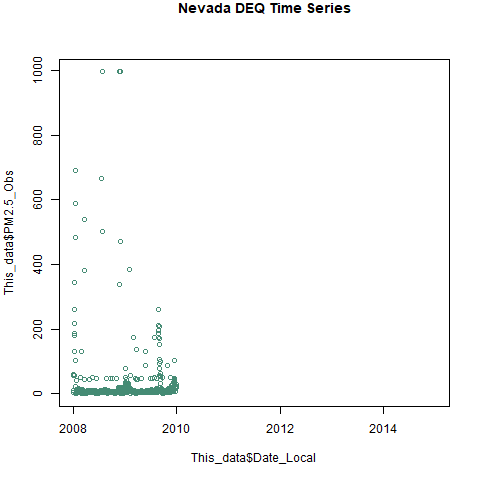
\includegraphics[width=0.77\textwidth]{Code_Outputs/NevadaDEQ_time_series.png} 
\caption{\label{fig:NevadaDEQTS}Nevada DEQ time series.} 
\end{figure} 
 
 % created from R code, not to be edited directly

\subsection{Utah Department of Environmental Quality }

\subsubsection*{Data Source}

\begin{itemize}[nolistsep]
\item \textbf{Contact} 
\item \textbf{Citation/Link} \url{http://www.airmonitoring.utah.gov/dataarchive/archpm25.htm}
\item \textbf{Data (local)} 
\item \textbf{Geographic Extent} Varies... 
\item \textbf{Temporal Extent} Hourly Value CSVs
\item \textbf{Acknowledgment} 
\end{itemize}

\subsubsection*{Brief Description} 
PM2.5 data from all monitoring stations in Utah

\subsubsection*{Notes} 
There was a lot of overlap with the EPA AQS data, so we took data only from the PM2.5 stations not reported by the EPA. 
This ended up being one or more of three stations (NP, HC, and RS) for 2009, 2010, 2012, and 2013.

Lat/Lon coordinates for site 49-049-0002 obtained from \url{http://www.airmonitoring.utah.gov/dataarchive/2009PM2.5.pdf}

\subsubsection*{File Formats} 

\subsubsection*{Data Filtering and Processing}

\subsubsection*{Final Variable(s)}

\subsubsection*{Methods}

\begin{enumerate}
\item 
\item
\end{enumerate}

\subsubsection*{Quality Control}

\subsubsection*{Script Names}

\begin{enumerate}
\item 
\end{enumerate}

\subsubsection*{Original Data File Names}

\begin{enumerate}
\item 
\item 
\end{enumerate}

\subsubsection*{Processed/Cleaned Data File Names}

\begin{enumerate}
\item 
\item 
\end{enumerate}



\subsection{Utah DEQ Plots}
\begin{figure} 
\centering 
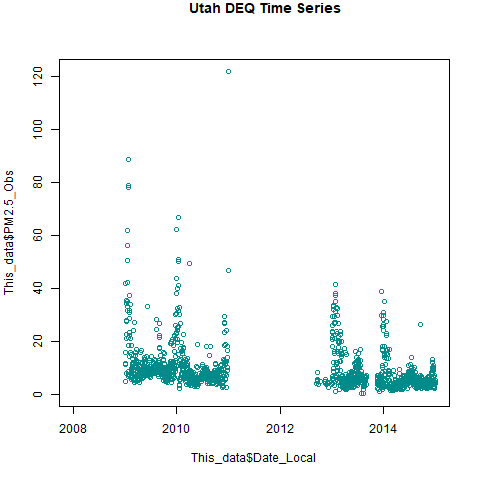
\includegraphics[width=0.77\textwidth]{Code_Outputs/UtahDEQ_time_series.png} 
\caption{\label{fig:UtahDEQTS}Utah DEQ time series.} 
\end{figure} 
 
 % created from R code, not to be edited directly

%%%%%%%%% AOD Data Sources %%%%%%%%%%%%%%%%%%%%%

\subsection{MODIS AOD}

\subsubsection*{Data Source}

\begin{itemize}[nolistsep]
\item \textbf{Contact}
\item \textbf{Citation/Link}
\item \textbf{Data (local)}
\item \textbf{Geographic Extent}
\item \textbf{Temporal Extent}
\item \textbf{Acknowledgment}
\end{itemize}

\subsubsection*{Brief Description}

We will use AOD estimates from the Deep Blue retrieval algorithm for AOD from the MODIS instrument on the NASA Terra and Aqua satellites (MOD04\_L2 and MYD04\_L2) \citep{Sayer2013}. The MODIS product is available twice daily at a 10 km spatial resolution for cloud-free scenes and is available longer than our 2008-2014  study period 
\citep{MODISMOD04L22017,MODISMYD04L22017}.  

AOD products use cloud filtering algorithms that often remove pixels in the center of the smoke plumes because they are assumed to be clouds due to high reflectivity \citep{kondragunta_revisions_2009}. Given that these can be in the middle of smoke plumes, often the locations most heavily impacted by smoke have missing data for a key variable, AOD. In our previous work in summer in California when rain clouds are incredibly rare, we could be confident that missing values not along the coast were not clouds. However, for this larger study region and time period, this will be a bigger challenge. We will attempt to isolate smoke plumes from true clouds using satellite imagery and smoke plume polygons from NOAA's Hazard Mapping System Fire Smoke Product  \citep{NOAAHazMap2017}. We will then estimate missing values within validated smoke plumes, but not within clouds, using radial basis functions as was done in our previous work \citep{Reid2015}. Radial basis functions are exact interpolation functions that will return observed AOD values where they exist but can interpolate higher values than nearby observations in missing locations, which is needed since the missing values were removed due to their high reflectivity \citep{Reid2015}.


\subsubsection*{Notes}

\subsubsection*{File Format} .hdf

\subsubsection*{Data Filtering and Processing}

\subsubsection*{Final Variable(s)}

\subsubsection*{Methods}

\begin{enumerate}
\item \underline{Step 1: Download the MODIS AOD data sets from both Terra and Aqua sensors:}\\\\
Using the \href{https://search.earthdata.nasa.gov/search?q=MOD04&ok=MOD04}{NASA EarthData online search tool}, search for the 'MOD04' (Terra) data set. Set temporal extent by drawing polygon and set spatial extent by adjusting the appropriate filter on the web interface. Select the collection and proceed to download data. For data download options, specify "Stage for Delivery" through the "FTPPull" distribution option. Specify the email address for orders to be sent to. Orders will be sent to your email with instructions on how to connect to the FTP server and pull the ordered data into your local workspace through the command line. Because the amount of data being requested is large, the orders will come through several separate emails. Repeat this step for the 'MYD04' (Aqua) data set. All of the raw downloaded data from this step will be in .hdf file format.
\item  \underline{Step 2: Set up file system for data processing:}\\\\ 
Create a directory locally named `collected\_data`. In this directory, make two child directories named "MOD04\_terra" and "MYD04\_aqua". Follow instructions in email to download data through FTP into the appropriate MODIS directory (`MOD04\_terra` or `MYD04\_aqua`) depending on whether the order is from the Terra or Aqua sensor. Create another directory locally named "processed\_data" at the same level as "collected\_data" (this is where the processed data will eventually go). This file naming convention is important because the python scripts that are run later depend on this hierarchy.
\item \underline{Step 3: Extract lat, long, and aod values from .hdf files and save into .csv files}\\\\
Run script `modis\_aod\_create\_csv\_file.py` (will need to change input and output filepath at top of script in order to match those of your local setup). This script will take all the .hdf files that you have downloaded and store the lat/long and aod value for non-null pixels. A .csv file will be created for each corresponding .hdf file and stored in your `processed\_data' folder.
\item \underline{Step 4: Create .shp file for each .csv file}\\\\
Run `modis\_aod\_convert\_csv\_to\_shapefile.py`. This script will read in the .csv files and convert them to .shp files using multiprocessing, which speeds up the process.

\item \underline{Step 5: Define projection to be US Albers Equal Area Conic}\\\\
Run `modis\_aod\_project\_to\_albers.py`. This script will define the projection of each .shp file to be US Albers Equal Area Conic (ESRI:102003).

\item \underline{Step 6: Combine .shp files for same date and convert to raster with 10km resolution}\\\\
Run `modis\_aod\_split\_shapefile\_by\_date.py`. This will combine all .shp files from the same date and then produce a raster for each with a 10km resolution.

\item \underline{Step 7: Clip the interpolated grids to study area}\\\\
Run `modis\_aod\_clip\_to\_study_area.py` which clips the interpolated grids to the 11 western states that is our study area

\item \underline{Step 8: Extract MODIS AOD value at EPA monitor locations}\\\\
Using ExtractValuesToPoints tool in ArcGIS.

\end{enumerate}

\subsubsection*{Quality Control}

\subsubsection*{Script Names}

\begin{enumerate}
\item modis\_aod\_create\_csv\_file.py
\item modis\_aod\_add\_utc\_to\_csv.py
\item modis\_aod\_merge\_csv\_files.py
\item modis\_aod\_split\_shapefile\_by\_date.py
\item modis\_aod\_create\_24hr\_daily\_averages.py
\end{enumerate}

\subsubsection*{Data File Names}

\begin{enumerate}
\item n/a
\end{enumerate}

\subsection{GASP-West AOD}

\subsubsection*{Data Source}

\begin{itemize}[nolistsep]
\item \textbf{Contact}
\item \textbf{Citation/Link}
\item \textbf{Data (local)}
\item \textbf{Geographic Extent}
\item \textbf{Temporal Extent}
\item \textbf{Acknowledgment}
\end{itemize}

\subsubsection*{Brief Description}

We will use AOD estimates from the Geostationary Operational Environmental Satellite West (GOES-West) Aerosol Smoke Product (GASP-West AOD). The GASP product is available at a 4 km resolution at nadir with retrievals every 30 minutes during daylight hours and is available from 2006 onward 
\citep{GASPAerosolProduct2017}.  

AOD products use cloud filtering algorithms that often remove pixels in the center of the smoke plumes because they are assumed to be clouds due to high reflectivity \citep{kondragunta_revisions_2009}. Given that these can be in the middle of smoke plumes, often the locations most heavily impacted by smoke have missing data for a key variable, AOD. In our previous work in summer in California when rain clouds are incredibly rare, we could be confident that missing values not along the coast were not clouds. However, for this larger study region and time period, this will be a bigger challenge. We will attempt to isolate smoke plumes from true clouds using satellite imagery and smoke plume polygons from NOAA's Hazard Mapping System Fire Smoke Product  \citep{NOAAHazMap2017}. We will then estimate missing values within validated smoke plumes, but not within clouds, using radial basis functions as was done in our previous work \citep{Reid2015}. Radial basis functions are exact interpolation functions that will return observed AOD values where they exist but can interpolate higher values than nearby observations in missing locations, which is needed since the missing values were removed due to their high reflectivity \citep{Reid2015}.

\subsubsection*{Notes}

websites: \url{https://www.ncdc.noaa.gov/data-access/satellite-data/satellite-data-access-datasets}  

\url{https://www.ncdc.noaa.gov/data-access/satellite-data/satellite-data-access-datasets}

Order form for data: \url{https://www.ncdc.noaa.gov/has/has.dsselect}

\url{https://www.ncdc.noaa.gov/doclib/index.php?choice=dsi&searchstring=3635&submitted=1&submitted=Search}


\subsubsection*{File Format}

\subsubsection*{Data Filtering and Processing}

\subsubsection*{Final Variable(s)}

\subsubsection*{Methods}

\begin{enumerate}
\item \underline{Download Data}\\\\
Navigate to NCEI's \href{https://www.ncdc.noaa.gov/has/has.dsselect}{Archive Information Request System (AIRS)}. Scroll down and click on 'Satellite' to expand menu. Click on 'Goes Products' to expand menu. Click on 'Order Data'. Select GOES-West for satellite ID, GASP-AOD-GZ for data type, and appropriate start and end date. Select "Yes" for Submit Batch. Enter email address and submit order. You will get emails later on with FTP links to your data. Run `Generic\_FTP\_download\_to\_S3.py` on an EC2 instance passing in the FTP url as the argument. This will download the data and upload it to S3 (and then delete it off the EC2 instance).
\end{enumerate}

\subsubsection*{Quality Control}

\subsubsection*{Script Names}

\begin{enumerate}
\item Generic\_FTP\_download\_to\_S3.py
\end{enumerate}

\subsubsection*{Data File Names}

\begin{enumerate}
\item 
\end{enumerate}


\subsection{MERRA-2}

\subsubsection*{Data Source}

\begin{itemize}[nolistsep]
\item \textbf{Contact} 
\item \textbf{Citation/Link} 
\item \textbf{Data (local)} 
\item \textbf{Geographic Extent} 
\item \textbf{Temporal Extent} 
\item \textbf{Acknowledgment} 
\end{itemize}

\subsubsection*{Brief Description}

%Provencal et al 2017 \citep{Provencal2017}

\subsubsection*{Notes}

\subsubsection*{File Formats} 

\subsubsection*{Data Filtering and Processing}

\subsubsection*{Final Variable(s)}

\subsubsection*{Methods}

\begin{enumerate}
\item 
\item
\end{enumerate}

\subsubsection*{Quality Control}

\subsubsection*{Script Names}

\begin{enumerate}
\item 
\end{enumerate}

\subsubsection*{Original Data File Names}

\begin{enumerate}
\item 
\item 
\end{enumerate}

\subsubsection*{Processed/Cleaned Data File Names}

\begin{enumerate}
\item 
\item 
\end{enumerate}

\subsection{MAIAC}

\subsubsection*{Data Source}

\begin{itemize}[nolistsep]
\item \textbf{Contact}
\item \textbf{Citation/Link}
\item \textbf{Data (local)}
\item \textbf{Geographic Extent}
\item \textbf{Temporal Extent}
\item \textbf{Acknowledgment}
\end{itemize}

\subsubsection*{Brief Description}



\subsubsection*{Notes}

\subsubsection*{File Format} 

\subsubsection*{Data Filtering and Processing}

\subsubsection*{Final Variable(s)}

\subsubsection*{Methods}

\begin{enumerate}
\item 

\end{enumerate}

\subsubsection*{Quality Control}

\subsubsection*{Script Names}

\begin{enumerate}
\item Contacted NASA DeepBlue team via email and was given the \href{ftp://dataportal.nccs.nasa.gov/DataRelease/}{FTP} site for their research data output. Public data set not yet available. But should be in several months under the name `MCD19`.
\end{enumerate}

\subsubsection*{Data File Names}

\begin{enumerate}
\item n/a
\end{enumerate}

%%%%%%%% Roadway Data %%%%%%%%%%%%%%%

\subsection{\texorpdfstring{National Highways Planning Network}

\subsubsection*{Data Source}

\begin{itemize}[nolistsep]
\item \textbf{Contact} 
\item \textbf{Citation/Link} \url{https://www.fhwa.dot.gov/planning/processes/tools/nhpn/index.cfm} 
\item \textbf{Data (local)} 
\item \textbf{Geographic Extent} Entire USA (including Alaska, Hawaii)
\item \textbf{Temporal Extent} Current
\item \textbf{Acknowledgment} 
\end{itemize}

\subsubsection*{Brief Description}
"Geospatial network database that contains line features representing just over 450,000 miles of highways in the United States"
... "In addition to the NHS [National Highway System], the NHPN covers all roads functionally classified as principal arterial and rural minor arterial."

\subsubsection*{Notes}

\subsubsection*{File Formats} 
Shapefile (with shp, dbf, shx, and prj)

\subsubsection*{Data Filtering and Processing}
Subset of only the western states in our study

\subsubsection*{Final Variable(s)}

\subsubsection*{Methods}

\begin{enumerate}
\item 
\item
\end{enumerate}

\subsubsection*{Quality Control}

\subsubsection*{Script Names}

\begin{enumerate}
\item 
\end{enumerate}

\subsubsection*{Original Data File Names}

\begin{enumerate}
\item 
\item 
\end{enumerate}

\subsubsection*{Processed/Cleaned Data File Names}

\begin{enumerate}
\item 
\item 
\end{enumerate}


%%%%%%%%% Satellite Fire Data Sources %%%%%%%%%%%

\subsection{MODIS Thermal Anomalies/Fire Daily L3 Global 1km (MOD14 and MYD14)}
\subsubsection*{Data Source}
\begin{itemize}[nolistsep]
\item \textbf{Contact}
\item \textbf{Citation/Link}
\item \textbf{Data (local)}
\item \textbf{Geographic Extent}
\item \textbf{Temporal Extent}
\item \textbf{Acknowledgment}
\end{itemize}
\subsubsection*{Brief Description}

We will collect data about fire detection locations, size, and fire radiative power from the MODIS Thermal Anomalies/Fire Daily L3 Global 1km (MOD14 and MYD14) \citep{Giglio2006,Hawbaker2017}. 
Using GIS techniques, we will create daily clusters of fire points and use these to calculate: (1) the distance to the nearest fire cluster by day and (2) the sum of Fire Radiative Power (FRP) of the nearest clusters of fires by day as it is likely that smoke levels are higher closer to fires. The MODIS product spans longer than our study period (2008-2014) at daily temporal resolution and has a spatial resolution of 1 km.

\subsubsection*{Notes}
\subsubsection*{File Format} .hdf
\subsubsection*{Data Filtering and Processing}
\subsubsection*{Final Variable(s)}
\subsubsection*{Methods}
\begin{enumerate}
\item Run script `MODIS\_FTP\_download.py` and pass two arguments: the first is the data set name and the second is the local directory path to save files to (i.e. "MOD14" "C:/Users/User/MOD14\_Downloads")
Update: `MODIS\_FTP\_download.py` is obsolete because NASA LAADS decomissioned their FTP site in favor of HTTPS. So, a new all-purpose script will need to be written to do this download that does HTTPS retrievals instead.
\end{enumerate}
\subsubsection*{Quality Control}
\subsubsection*{Script Names}
\begin{enumerate}
\item MODIS\_FTP\_Download.py
\end{enumerate}
\subsubsection*{Data File Names}
\begin{enumerate}
\item n/a
\end{enumerate}

\subsection{Landsat-derived burned area essential climate variable (BAECV) fire activity data}
\subsubsection*{Data Source}
\begin{itemize}[nolistsep]
\item \textbf{Contact}
\item \textbf{Citation/Link}
\item \textbf{Data (local)}
\item \textbf{Geographic Extent}
\item \textbf{Temporal Extent}
\item \textbf{Acknowledgment}
\end{itemize}
\subsubsection*{Brief Description}

We will collect data about fire detection locations, size, and fire radiative power from the Landsat-derived burned area essential climate variable (BAECV) fire activity data, 
\citep{MODISBurnArea}. 
Using GIS techniques, we will create daily clusters of fire points and use these to calculate: (1) the distance to the nearest fire cluster by day and (2) the sum of Fire Radiative Power (FRP) of the nearest clusters of fires by day as it is likely that smoke levels are higher closer to fires.  The BAECV can detect fires larger than 4 km\textsuperscript{2} and provides an estimate of the date of the fire and is available from 1984-2015. 

\subsubsection*{Notes}
\subsubsection*{File Format} .shp
\subsubsection*{Data Filtering and Processing}
\subsubsection*{Final Variable(s)}
\subsubsection*{Methods}
\begin{enumerate}
\item BAECV data set already downloaded by EarthLab fire group. Navigate to the `earthlab-ls-fire` S3 bucket, then the v1.1 subdirectory. Here you will find yearly .tar.gz files. Have not spent time decompressing files and exploring data yet but my guess is that within each yearly file, we will find more detailed, daily burn data.
\end{enumerate}
\subsubsection*{Quality Control}
\subsubsection*{Script Names}
\begin{enumerate}
\item n/a
\end{enumerate}
\subsubsection*{Data File Names}
\begin{enumerate}
\item n/a
\end{enumerate}

\subsection{MODIS/Terra and Aqua Burned Area Monthly L3 Global 500 m SIN Grid V006 (MCD64A1) }
\subsubsection*{Data Source}
\begin{itemize}[nolistsep]
\item \textbf{Contact}
\item \textbf{Citation/Link}
\item \textbf{Data (local)}
\item \textbf{Geographic Extent}
\item \textbf{Temporal Extent}
\item \textbf{Acknowledgment}
\end{itemize}
\subsubsection*{Brief Description}

We will collect data about fire detection locations, size, and fire radiative power from MODIS/Terra and Aqua Burned Area Monthly L3 Global 500 m SIN Grid V006 (MCD64A1) 
\citep{Schroeder2014}. % check if this is the right citation
Using GIS techniques, we will create daily clusters of fire points and use these to calculate: (1) the distance to the nearest fire cluster by day and (2) the sum of Fire Radiative Power (FRP) of the nearest clusters of fires by day as it is likely that smoke levels are higher closer to fires.

\subsubsection*{Notes}
\subsubsection*{File Format} .hdf
\subsubsection*{Data Filtering and Processing}
\subsubsection*{Final Variable(s)}
\subsubsection*{Methods}
\begin{enumerate}
\item Run script and pass two arguments: the first is the data set name and the second is the local directory path to save files to (i.e. "MCD64A1" "C:/Users/User/MCD64A1\_Downloads")
\end{enumerate}
\subsubsection*{Quality Control}
\subsubsection*{Script Names}
\begin{enumerate}
\item MODIS\_FTP\_Download.py
\end{enumerate}
\subsubsection*{Data File Names}
\begin{enumerate}
\item 
\end{enumerate}

%%%%%%%%% VIIRS Infrared Data Source %%%%%%%%%%

\subsection{Visible Infrared Imaging Radiometer Suite (VIIRS) (VNP14IMGTDL\_NRT) }
\subsubsection*{Data Source}
\begin{itemize}[nolistsep]
\item \textbf{Contact}
\item \textbf{Citation/Link}
\item \textbf{Data (local)}
\item \textbf{Geographic Extent}
\item \textbf{Temporal Extent}
\item \textbf{Acknowledgment}
\end{itemize}
\subsubsection*{Brief Description}

We will collect data about fire detection locations, size, and fire radiative power from the Visible Infrared Imaging Radiometer Suite (VIIRS) (VNP14IMGTDL\_NRT) 
\citep{Schroeder2014}. % not sure if that's the right citation
Using GIS techniques, we will create daily clusters of fire points and use these to calculate: (1) the distance to the nearest fire cluster by day and (2) the sum of Fire Radiative Power (FRP) of the nearest clusters of fires by day as it is likely that smoke levels are higher closer to fires. The MODIS product spans longer than our study period (2008-2014) at daily temporal resolution and has a spatial resolution of 1 km. VIIRS was launched in 2011 and has 12 h temporal resolution with 750 m resolution. The BAECV can detect fires larger than 4 km\textsuperscript{2} and provides an estimate of the date of the fire and is available from 1984-2015. 

\subsubsection*{Notes}
\subsubsection*{File Format} .csv
\subsubsection*{Data Filtering and Processing}
\subsubsection*{Final Variable(s)}
\subsubsection*{Methods}
\begin{enumerate}
\item Go to the \href{https://firms.modaps.eosdis.nasa.gov/download/}{NASA EarthData Fire Information for Resource Management System (FIRMS) online tool} and navigate to the Archive section. Click 'Create New Request' and specify spatial and temporal resolution. Also choose 'VIIRS' from Fire Data Source. Choose 'csv' as file type and enter email address. Wait for email, which will contain a .zip file with the data.
\end{enumerate}
\subsubsection*{Quality Control}
\subsubsection*{Script Names}
\begin{enumerate}
\item n/a
\end{enumerate}
\subsubsection*{Data File Names}
\begin{enumerate}
\item fire\_archive\_V1\_2770.csv
\end{enumerate}


%%%%%%%%% Land Surface Attributes %%%%%%%%%%%%%

\subsection{Classified land cover information from the Landsat-derived NLCD 2011}
\subsubsection*{Data Source}
\begin{itemize}[nolistsep]
\item \textbf{Contact}
\item \textbf{Citation/Link}
\item \textbf{Data (local)}
\item \textbf{Geographic Extent}
\item \textbf{Temporal Extent}
\item \textbf{Acknowledgment}
\end{itemize}
\subsubsection*{Brief Description}

Classified land cover information from the Landsat-derived NLCD 2011 
\citep{Homer2017} will be used to calculate estimates of the percentage of urban development (codes 22, 23, and 24), agriculture (codes 81 and 82), and vegetated area other than agricultural land (codes 21, 41, 42, 43, 52, and 71) within buffer radii of 100 m, 250 m, 500 m, and 1000 m around each monitor. The buffer distance that is most highly correlated with PM\textsubscript{2.5} will be entered into each model. NLCD 2011 has a spatial resolution of 30 m and uses circa 2011 Landsat satellite data. 

\subsubsection*{Notes}
Use special Albers projection (ESRI 102003) to create the buffers (can import the projection from existing file on S3).
\subsubsection*{File Format} .shp
\subsubsection*{Data Filtering and Processing}
\subsubsection*{Final Variable(s)}
\subsubsection*{Methods}
\begin{enumerate}
\item Navigate to the \href{https://viewer.nationalmap.gov/basic/}{National Map Viewer} and find products for "National Land Cover Database (NLCD)" at the National extent. From the search results, download "NLCD 2011 Land Cover (2011 Edition, amended 2014)". This will download a zipfile with the data.
\item Run nlcd\_process.py with the required arguments. This script computes zonal statistics between a buffer shp file and an classified raster tif (in our use case, a reclassified NLCD raster). The computed value is percent area of developed high density land cover in each buffer. The output is another csv, which is the input csv with an an extra column denoting the data.
Note: the buffer shp file used in this study consisted of 1km, 5km, and 10km radius buffers using planar buffering.
\end{enumerate}
\subsubsection*{Quality Control}
\subsubsection*{Script Names}
\begin{enumerate}
\item nlcd\_process.py
\end{enumerate}
\subsubsection*{Data File Names}
\begin{enumerate}
\item n/a
\end{enumerate}


\subsection{MODIS Snow Cover Daily L3 Global 500m Grid, Version 6 (MOD10A1 and MYD10A1)}
\subsubsection*{Data Source}
\begin{itemize}[nolistsep]
\item \textbf{Contact}
\item \textbf{Citation/Link}
\item \textbf{Data (local)}
\item \textbf{Geographic Extent}
\item \textbf{Temporal Extent}
\item \textbf{Acknowledgment}
\end{itemize}
\subsubsection*{Brief Description}

We will use snow cover data from the MODIS Snow Cover Daily L3 Global 500m Grid, Version 6 (MOD10A1 and MYD10A1) \citep{Hall2016} because snow coverage is a known contributor to wintertime PM\textsubscript{2.5} concentrations in mountain valleys \citep{Whiteman2014}. Daily MOD10A1 and MYD10A1 data are available since 2002 and have 500 m spatial resolution. 

\subsubsection*{Notes}
\subsubsection*{File Format}
\subsubsection*{Data Filtering and Processing}
\subsubsection*{Final Variable(s)}
\subsubsection*{Methods}
\begin{enumerate}
\item \underline{Step 1: Download the MODIS AOD data sets from both Terra and Aqua sensors:}\\\\
Using the \href{https://search.earthdata.nasa.gov/}{NASA EarthData online search tool}, search for the 'MOD10A1' (Terra) data set. Set temporal extent by drawing polygon and set spatial extent by adjusting the appropriate filter on the web interface. Select the collection and proceed to download data. For data download options, specify "Stage for Delivery" through the "FTPPull" distribution option. Specify the email address for orders to be sent to. Orders will be sent to your email with instructions on how to connect to the FTP server and pull the ordered data into your local workspace through the command line. Because the amount of data being requested is large, the orders will come through several separate emails. Repeat this step for the 'MYD10A1' (Aqua) data set. All of the raw downloaded data from this step will be in .hdf file format.
\end{enumerate}
\subsubsection*{Quality Control}
\subsubsection*{Script Names}
\begin{enumerate}
\item 
\end{enumerate}
\subsubsection*{Data File Names}
\begin{enumerate}
\item 
\end{enumerate}

	\subsubsection{Elevation}
\subsubsection*{Data Source}
\begin{itemize}[nolistsep]
\item \textbf{Contact}
\item \textbf{Citation/Link}
\item \textbf{Data (local)}
\item \textbf{Geographic Extent}
\item \textbf{Temporal Extent}
\item \textbf{Acknowledgment}
\end{itemize}
\subsubsection*{Brief Description}

Elevation can influence PM\textsubscript{2.5} concentrations; for example, PM\textsubscript{2.5} can accumulate in mountain valleys during persistent cold air pools 
(commonly referred to as inversions) 
during winter \citep{Whiteman2014}. We will get elevation data from the 3D Elevation Program, which has resolution of 1 arc-second. This resolution is approximately 30 m north/south and varies east/west with latitude \citep{USGSElevation2017}.

\subsubsection*{Notes}
\subsubsection*{File Format}
\subsubsection*{Data Filtering and Processing}
\subsubsection*{Final Variable(s)}
\subsubsection*{Methods}
\begin{enumerate}
%\item Navigate to the \href{https://viewer.nationalmap.gov/basic/?basemap=b1&category=ned,nedsrc&title=3DEP%20View}{National Map Viewer} site and find products for Elevation Products (3DEP), 1 arc-second DEM, IMG file format. Once results are returned, select "Save as Text", which will download a text file containing server links to each NED tile.
\item Navigate to the \url{https://viewer.nationalmap.gov/basic/?basemap=b1&category=ned,nedsrc&title=3DEP View}{National Map Viewer} site and find products for Elevation Products (3DEP), 1 arc-second DEM, IMG file format. Once results are returned, select "Save as Text", which will download a text file containing server links to each NED tile.

\item Download the data using the \href{https://github.com/earthlab/estimate-pm25/blob/master/download-earth-observations/NED/download_tiles.py}{download\_tiles.py} script, which will access the text file that you just downloaded. 

\item Extract the elevation values using the \href{https://github.com/earthlab/estimate-pm25/blob/master/download-earth-observations/NED/extract_values_to_points.py}{extract\_values\_to\_points.py} script. Step-by-step instructions:
	\begin{enumerate}
	\item Start t2.medium EC2 instance on AWS with 250 BG storage
	\item docker pull earthlab/estimate-pm25
	\item docker run -d earthlab/estimate-pm25
	\item docker ps
	\item docker exec -it [docker\_name] /bin/bash
	\item aws configure
	\item mkdir NED
	\item cd NED
	\item mkdir data 
	\item aws s3 cp s3://earthlab-reid-group/NED/data/ /home/jovyan/NED/data/ --recursive 
		\begin{enumerate}
		\item This step takes a few hours
		\end{enumerate}
	\item aws s3 cp s3://earthlab-reid-group/Processed\_Data/PM25\_Locations\_Dates/ /home/jovyan/NED/ --recursive
	\item git clone https://github.com/earthlab/estimate-pm25.git
	\item cd estimate-pm25
	\item cd download-earth-observations/NED/
	\item python extract\_values\_to_\points.py --NED\_directory "/home/jovyan/NED/data/" --input\_csv\_file "/home/jovyan/NED/Part\_e\_not\_in\_bd\_Locations.csv" --output\_csv\_file "/home/jovyan/NED/ned\_part\_e\_not\_bd\_extract.csv"
	\item See also: \url{https://docs.google.com/document/d/1IysKoAS8l1WH6nN4IksWe9MWqNZEOG5DQD9DYGjOcX8/edit?usp=sharing}
	\end{enumerate}




\end{enumerate}
\subsubsection*{Quality Control}
\subsubsection*{Script Names}
\begin{enumerate}
\item download\_tiles.py
\item extract\_values\_to\_points.py
\end{enumerate}
\subsubsection*{Data File Names}
\begin{enumerate}
\item n/a
\end{enumerate}

%%%%%%%% Atmospheric Data %%%%%%%%%%%%%

\subsection{Meteorological Data}
%\subsubsection*{Data Source} NCEP North American Regional Reanalysis (NARR) from NCAR
\subsubsection*{Data Source} North American Mesoscale, Analysis (NAM)
\begin{itemize}[nolistsep]
\item \textbf{Contact} %Chi-Fan Shih, chifan@ucar.edu
%\item \textbf{Citation/Link}  \url{https://rda.ucar.edu}, \url{https://rda.ucar.edu/datasets/ds608.0/}.
\item \textbf{Citation/Link} \url{https://www.ncdc.noaa.gov/data-access/model-data/model-datasets/north-american-mesoscale-forecast-system-nam},  \url{https://nomads.ncdc.noaa.gov/data/namanl/}
%\item \textbf{Data (local)} May 10, 2018
\item \textbf{Geographic Extent} North America
\item \textbf{Temporal Extent} Available March, 2004 - 2018
\item \textbf{Acknowledgment}
\end{itemize}
\subsubsection*{Brief Description}

%We will obtain meteorological data from the National Centers for Environmental Prediction (NCEP) North American Regional Reanalysis (NARR) \citep{Mesinger2006,NCEPReanalysis2005} because it includes all of the standard meteorological variables but also has planetary boundary layer height, which has proved to be an important variable for converting AOD to PM\textsubscript{2.5} \citep{liu_estimating_2005}. We will calculate 24-hour averages from 3-hourly data for temperature, relative humidity, sea level pressure, surface pressure, planetary boundary layer height, dew point temperature, precipitation, and the U and V components of wind speed. NARR has 32 km resolution and is available from 1979 onward. 

We will obtain meteorological data from the North American Mesoscale, Analysis (NAM) because it includes all of the standard meteorological variables, including planetary boundary layer height, which has proved to be an important variable for converting AOD to PM\textsubscript{2.5} \citep{liu_estimating_2005}. We will calculate 24-hour averages from 6-hourly data for temperature, relative humidity, sea livel pressure, surface pressure, planetary boundary layer height, dew point temperature, precipitation, snow coverage, and the U and V components of wind speed. NAM has 12 km resolution and is available 2004 onward.

\subsubsection*{Notes}

%We contacted Chi-Fan Shih at NCAR. She emailed us a link to the requested data (link is only valid for 11 days). The data is 28.31 G, and the website provides a few options for how to download the data. We chose the ``Perl download script'' button, which generates a short perl script specific to the requested data. To use this, we downloaded Perl \url{http://strawberryperl.com/} (see also \url{https://www.perl.org/}). The generated perl script calls wget( \url{https://www.gnu.org/software/wget/})

\subsubsection*{File Format}

Prior to 2018, the files are in *.grb (``grib1'') format, while 2018 data is in *.grb2 (``grib2'') format.

%.grb.tar
Resources about this file type: 
\begin{itemize}
\item rNOMADS is an R package for accessing grb* files. It is mostly geared for grib2 files. \url{https://cran.r-project.org/web/packages/rNOMADS/rNOMADS.pdf}
\item Explanation of what grib files are: \url{http://www.cpc.ncep.noaa.gov/products/wesley/reading_grib.html}, 
\item wgrib program information: \url{http://www.cpc.ncep.noaa.gov/products/wesley/wgrib.html}


\end{itemize}

If the resources above are insufficient for accessing the grb files, consider using GrADS: \url{http://www.cpc.ncep.noaa.gov/products/wesley/links_grads.html}

\subsubsection*{Data Filtering and Processing}

\begin{enumerate}

\item Use the earthlab/r-reidgroup docker image, which has wgrib and wgrib \url{http://www.cpc.ncep.noaa.gov/products/wesley/wgrib.html} and wgrib2 \url{http://www.cpc.ncep.noaa.gov/products/wesley/wgrib2/} installed on it.

\item Process\_NAM\_data\_step1.R reads in Locations\_Dates\_of\_PM25\_Obs\_DeDuplicate.csv and outputs Locations\_Dates\_of\_PM25\_Obs\_DeDuplicate_wNextDay.csv, which includes the next day for each location/day listed in the first file. The purpose of this is so all of the necessary NAM files can be processed. UTC dates can go into the next day for western US time zones. Calls add\_next\_day\_date\_loc\_function.R.

\item Process\_NAM\_data.R downloads NAM files (one at a time), extracts relevant data, and deletes the original NAM data. (All of the NAM files together would be about 1.6 Tb.) Process\_NAM\_data.R uses these input files and R packages and functions:
	\begin{enumerate}
	\item Locations\_Dates\_of\_PM25\_Obs\_DeDuplicate.csv - Data file with dates (local) and locations where you want the NAM data
	\item MeteoVariablesNAM.csv - listing of meteorological variables to be extracted from NAM data
	\item rNOMADS package (which calls wgrib and wgrib2) \url{https://cran.r-project.org/web/packages/rNOMADS/rNOMADS.pdf}
	\item To Do: set it up to use grb1to2\_MMM.pl to convert grib1 to grib2 files - need Max's help with permissions error
	\item extract\_NAM\_data\_function.R
	\item add\_next\_day\_date\_loc\_function.R used in extract\_NAM\_data\_function.R
	\item which\_type\_of\_grib\_file\_function.R used in extract\_NAM\_data\_function.R
	\end{enumerate}

\item To Do: Process\_NAM\_data.R will output 4 data frames, one for each run time for the NAM model in UTC time (00, 06, 12, 18).

\item To Do: Merge\_NAM\_times.R will merge the 4 time steps to give a 24-hr summary. Min, max, mean, etc. is set in MeteoVariabesNAM.csv.

%\item download .grb.tar files (requested from Chi-Fan Shih, who sent a link that was good for about 2 weeks)

%\item untar files. The files came as yyyy.grb.tar where yyyy are years 2008-2014. To un-tar the files, open GitBash, and type: tar -xvf 2008.grb.tar This will create a folder called 2008 with many .grb files. Repeat for the other years. See also \url{https://labcit.ligo.caltech.edu/~ethrane/Resources/UNIX/}

%\item Download cygwin (windows only) (to be able to compile wgrib2) from \url{https://www.cygwin.com/}. Chose \url{http://mirrors.xmission.com} as the download site (don't think it matters), searched make and then clicked ``Default'' on all the options so they became ``Install'', see \url{https://stackoverflow.com/questions/4825317/cygwin-make-help} and \url{https://stackoverflow.com/questions/17710209/how-to-run-make-from-cygwin-environment}.
%	\begin{enumerate}
%	\item go to \url{https://www.cygwin.com/}
%	\item click on ``setup-x86\_64.exe'', save file, run
%	\item when selecting components, click on Devel then find ``make'' and change ``Skip'' to ``Install'' (or click ``Skip'' so it changes to 4.1-1''
%	\end{enumerate}

%\item download gcc compiler from \url{https://sourceforge.net/projects/mingw-w64/}

%\item download gfortran compiler from \url{http://gcc.gnu.org/wiki/GFortranBinariesWindows}

%\item Download wgrib2 from here: \url{ftp://ftp.cpc.ncep.noaa.gov/wd51we/wgrib2/wgrib2.tgz} Instructions for wgrib2 at \url{http://www.cpc.ncep.noaa.gov/products/wesley/wgrib2/compile_questions.html} indicate the for ``For Windows 10, you can use WSL and the Ubuntu compilers. Use the generic linux instructions '' %(uses cygwin)... need to download gcc compiler
%	\begin{enumerate}
%		\item \url{https://dev.openttdcoop.org/projects/home/wiki/Setting_up_a_Windows_compile_environment_using_WSL}
%	\end{enumerate}

%\item Download wgrib 

%\item alternatively trying to download grads, which may have compiled versions of wgrib and wgrib2 in it \url{http://opengrads.org/} ... didn't work

%\item use rNOMADS R package. It looks like the rNOMADS R package can read .grb files \url{https://cran.r-project.org/web/packages/rNOMADS/rNOMADS.pdf}. rNOMADS calls external routines called wgrib2 .

%\item \url{ftp://ftp.cpc.ncep.noaa.gov/wd51we/wgrib/readme}

%\item Octet code info: \url{http://www.nco.ncep.noaa.gov/pmb/docs/on388/section1.html}

%\item \url{https://rda.ucar.edu/docs/formats/grib/gribdoc/pds.html}

\end{enumerate}

\subsubsection*{Final Variable(s)}
\subsubsection*{Methods}
\begin{enumerate}
\item 
\item
\end{enumerate}
\subsubsection*{Quality Control}
\subsubsection*{Script Names}
\begin{enumerate}
\item 
\end{enumerate}
\subsubsection*{Data File Names}
\begin{enumerate}
\item 
\end{enumerate} 

%\section{North American Mesoscale, Analysis}

%\begin{enumerate}
%\item \url{https://www.ncdc.noaa.gov/data-access/model-data/model-datasets/north-american-mesoscale-forecast-system-nam}

%\end{enumerate}

%\section{GFS}

%\begin{enumerate}
%\item \url{https://www.ncdc.noaa.gov/data-access/model-data/model-datasets/global-forcast-system-gfs}
%\item 0.5 degree resolution, which is about 55 km %(\url{https://www.vets.ucar.edu/vg/Climate_Model_Resolution%20%20/index.html})

%\end{enumerate}

\subsection{Dust Storms}
\subsubsection*{Data Source}
\begin{itemize}[nolistsep]
\item \textbf{Contact}
\item \textbf{Citation/Link}
\item \textbf{Data (local)}
\item \textbf{Geographic Extent}
\item \textbf{Temporal Extent}
\item \textbf{Acknowledgment}
\end{itemize}
\subsubsection*{Brief Description}

Dust storm records will be included in the machine learning algorithm because they can be a significant indicator of airborne particulate matter from sources other than fires. Dust storm records are available from 1993-2017. The spatial resolution varies, but includes either forecast zone or county  \citep{NWSstorms2017,NWSrecordhistory2017,NWSInstructions2016}.

\subsubsection*{Notes}
\subsubsection*{File Format}
\subsubsection*{Data Filtering and Processing}
\subsubsection*{Final Variable(s)}
\subsubsection*{Methods}
\begin{enumerate}
\item 
\item
\end{enumerate}
\subsubsection*{Quality Control}
\subsubsection*{Script Names}
\begin{enumerate}
\item 
\end{enumerate}
\subsubsection*{Data File Names}
\begin{enumerate}
\item 
\end{enumerate}

\include{Traffic_Roads}

%%%%%%%%%%%% CAMx Data Sources %%%%%%%%%%%%%%%%%%

\section{Data Sources for CAMx Modeling of Source-Attributed Air Quality Modeling}\label{sec:CAMxDataSources}

For meteorological inputs, the CAMx modeling will use archived daily 27-km Advanced Research Weather Research and Forecasting (WRF-ARW) grids available via NOAA Real-time Environmental Applications and Display sYstem (READY) servers for the entire study area and time period \citep{Wang2007,Rolph2017}. For the study years 2008-2012 and 2014, we will use fire emissions datasets prepared by the Western Regional Air Partnership (WRAP) and the National Emissions Inventory (NEI) \citep{EPANEI2017} based on aggregated source-tagged fire occurrence data sources, the FCCS \citep{Ottmar2007}, and Consume \citep{Prichard2009}
modeling. For the study year 2013, we will prepare a fire emissions dataset using the same aggregated source-tagged fire occurrence data sources and FCCS/Consume modeling framework in the NASA-funded  Wildland Fire Emissions Information System (WFEIS) \citep{WFEIS2017} developed by Co-I's French and Billmire \citep{French2014}. Fire occurrence datasets include MODIS  (MOD14/MYD14 and MCD64A1) and  VIIRS (VNP14IMGTDL\_NRT) fire data products \citep{Giglio2006,MODISBurnArea,Schroeder2014}. 
For non-fire emissions during the entire study period, we will use the dataset prepared by WRAP for year 2008.

Look into using spot forecasts to help distinguish between wild and prescribed fires: \url{http://www.weather.gov/spot/monitor/}

%%%%%%%%%%% CAMx Modeling

\section{CAMx Modeling}


%%%%%%%%%%%%%% Data processing %%%%%%%%%%%%%%%%%%%%%%%

%\subsection{$\textrm{PM}_{2.5}$ data}%{Compiling Data}

\subsubsection{Processing $\textrm{PM}_{2.5}$ data}

Below are the scripts that process and compile the PM\textsubscript{2.5} data. The ``*'' in each of the file names refers to the current ``processed\_data\_version'' (set in general\_project\_functions.R)  since compiling the data is an ongoing process. 

\begin{enumerate}[nolistsep]
\item \textul{Script1\_Install\_Pkgs.R} >> install packages

\item \textul{Process\_PM25\_data\_step1.R} >> compiles the various PM\textsubscript{2.5} data sources into a single data frame. The only eliminations of data are geographic, to remove states that are not in our study area. Update time frame of study if necessary. The output from this script is a csv file and sink .txt for each  PM\textsubscript{2.5} data source as well as a file with all of the PM\textsubscript{2.5} data sources merged together (``PM25\_Step1\_part\_*.csv''). This script takes about 6 minutes to run on a laptop. %This script creates a main data file as well as a csv of data for each PM2.5 data source and a text file describing the data:
\begin{enumerate}
\item PM25\_Step1\_part\_*.csv (the main data file)
\item PM25\_CARB\_Step1\_part\_*.csv
\item PM25\_CARB\_Step1\_part\_*\_combining\_sink.txt
\item PM25\_EPA\_Step1\_part\_*.csv
\item PM25\_EPA\_Step1\_part\_*\_combining\_sink.txt
\item PM25\_FireCacheDRI\_Step1\_part\_*.csv
\item PM25\_FireCacheDRI\_Step1\_part\_*\_combining\_sink.txt
\item PM25\_IMPRHR2MF88101\_10010\_Step1\_part\_*.csv
\item PM25\_IMPRHR2MF88101\_10010\_Step1\_part\_*\_combining\_sink.txt
\item PM25\_IMPRHR2RCFM88401\_10010\_Step1\_part\_*.csv
\item PM25\_IMPRHR2RCFM88401\_10010\_Step1\_part\_*\_combining\_sink.txt
\item PM25\_IMPRHR3MF88101\_10006\_Step1\_part\_*.csv
\item PM25\_IMPRHR3MF88101\_10006\_Step1\_part\_*\_combining\_sink.txt
\item PM25\_PCAPS\_Step1\_part\_*.csv
\item PM25\_PCAPS\_Step1\_part\_*\_combining\_sink.txt
\item PM25\_UintahBasin\_Step1\_part\_*.csv
\item PM25\_UintahBasin\_Step1\_part\_*\_combining\_sink.txt
\item PM25\_UtahDEQ\_Step1\_part\_*.csv
\item PM25\_UtahDEQ\_Step1\_part\_*\_combining\_sink.txt
\end{enumerate}

Notes that are useful when incorporating new data:
\begin{enumerate}
\item \textbf{Federal Land Manager Database (IMPROVE) data:} Download data as described in Section \ref{IMPROVE}. Edit ``skip\_n\_files'' in process\_PM25\_parallel\_wrapper\_function.R so that FMLEdata\_Parameter\_MetaData will load the row with the header `DatasetID, Parameter, Code, AQSCode, Units, Description' for each IMPROVE file.
\end{enumerate}

	\begin{enumerate}
	\item For DRI data, put in flags for voltage data outside the range 11-17 V. (These thresholds are somewhat arbitrary, but it was noticed that when the voltage was outside this range, the PM\textsubscript{2.5} concentrations were often absurdly high, e.g., greater than 24,000 ug/m3.
	\end{enumerate}

\item \textul{Process\_PM25\_data\_step2.R} >> cleans the data. This script takes about 5 minutes on a laptop. This script outputs the following files: 
	\begin{enumerate}[nolistsep]
	\item PM25\_Step2\_part\_*.csv (main cleaned data file)
	\item PM25\_Step2\_part\_*\_sink.txt (description and summaries of the data at each step of the quality cutting)
	\item PM25\_Step2\_part\_*\_Locations.csv (list of unique locations from main cleaned data file)
	\item PM25\_Step2\_part\_*\_Locations\_Dates.csv (list of unique locations/dates from main cleaned data file)
	\item Data\_Removed\_in\_PM25\_Step2\_part\_*.csv (list of unique locations from main cleaned data file)
	\end{enumerate}
The following is a list of the quality cuts and changes made to the data:
	\begin{enumerate}[nolistsep]
	\item Replace ``UNKNOWN'' datum in EPA data with ``NAD27'' per Colleen's advice.
	\item Remove negative and NA PM\textsubscript{2.5} concentrations. This includes removing all data for a monitor on a given day if any of the hourly observations were negative.
	\item For the hourly data, remove monitor-days that do not have at least 18/24 observations.
	\item For DRI data, remove data with voltage flags (which includes flags that came with the data and flags that were put in because the battery voltage was outside the range 11-17 V.
	\item For DRI data, remove data at or below 0 L/min for flow. Think about whether a minimum value of flow should be set (higher than zero).
	\item June 6, 2014 24-hr average PM\textsubscript{2.5} concentration from monitor ``Smoke NCFS E-BAM \#1'' (Fire\_Cache\_Smoke\_DRI\_Smoke\_NCFS\_E\_BAM\_N1.csv) is 24,203 ug/m3. There's nothing apparent wrong with the hourly data, however, this is the only day of data that made it through the other quality checks from this data file. This suggests that this monitor is suspect, and will be removed.
	\item Remove data points with lat/lon outside this box: (50,-126) to (25,-101). These values are defined in general\_project\_functions.R. %-93) 
	\item Remove data outside the study period (defined in general\_project\_functions.R).
	\item Remove data with ``Event\_Type'' = ``Excluded''
	\item Remove data with more than 0.001 degrees variation in Lat/lon within a day
	\item Remove data from monitor ``USFS R2-265'' (Fire\_Cache\_Smoke\_USFS\_R2-265.csv) between October 2016 - May 2017. The concentrations (some higher than 65,000,000 ug/m3) and the behavior of the concentrations (frequently changing by exactly 1000 ug/m3 from one hour to the next) are unrealistic. The data outside this time frame look more reasonable.
	\item Remove data from monitor ``USFS R2-264'' (Fire\_Cache\_Smoke\_USFS\_R2-264.csv") between October 2016 - October 2017. The behavior of the concentrations (frequently changing by exactly 1000 ug/m3 from one hour to the next) are unrealistic. The data outside this time frame look more reasonable.
	\item Remove data from monitor ``FWS Smoke \#1'' (Fire\_Cache\_Smoke\_DRI\_FWS\_Smoke\_N1.csv) between February 11-14, 2017. The behavior of the concentrations (frequently changing by exactly 1000 ug/m3 from one hour to the next) are unrealistic. The data outside this time frame look more reasonable.
	\item Remove data from monitor ``Smoke \#22'' (Fire\_Cache\_Smoke\_DRI\_Smoke\_22.csv) on June 15, 2012. The behavior of the concentrations (frequently changing by exactly 1000 ug/m3 from one hour to the next) are unrealistic. The data outside this time frame look more reasonable.


	% if the monitor is near a fire, the air temperature could be quite high \item \textbf{To Do} think about making cuts on any unrealistic air temperatures for DRI data
	%seems unnecessary since both are removed \item \textbf{To Do} need to convert missing values that have a -9999 etc to NA value
	%seems unnecessary \item \textbf{To Do} merge "24-HR BLK AVG" and "24 HOUR" data together in Sample Duration variable
	%One site in Maricopa, AZ has some data points with an observation count of 2 and Observation Percent of 200. The data looks fine otherwise, so I'll keep it. %\item \textbf{To Do} figure out why Observation percent has a max value of 200\%
	% this data point was removed with the other quality cuts %\item \textbf{To Do} figure out if max AQI value of 546 is reasonable
	%can't find 20:00 in the wrong columns - maybe those versions were over-written if we downloaded the files again, not sure. %\item \textbf{To Do} Some DRI files looked like they had hour 20:00 data shifted a couple of columns - look into this and fix it.
	%I think I did this in later scripts. %\item \textbf{To Do} Finish filling in Year, month, day information based on date
	%\item \textbf{To Do} look over summary() output and plots of every variable and determine if any other cuts are necessary
	\end{enumerate}

\item \textul{Process\_PM25\_data\_step3.R} >> convert all PM2.5 data to the same datum (NAD83) and project coordinates. Take the reprojected location info and put it into the data frame with the daily PM\textsubscript{2.5} data. This script also rounds all lat/lon info to 5 digits. This script takes about 3 minutes on a laptop. This script outputs these files:

\begin{enumerate}[nolistsep]
\item PM25\_Step3\_part\_*\_Projected.csv (main data file)
\item PM25\_Step3\_part\_*\_Locations\_Projected\_include\_old\_projection.csv
\item PM25\_Step3\_part\_*\_Locations\_Projected.csv
\item PM25\_Step3\_part\_*\_Locations\_Dates\_Projected\_include\_old\_projection.csv
\item PM25\_Step3\_part\_*\_Locations\_Dates\_Projected.csv
\end{enumerate}

%\item \textul{Define\_directories.R} >> (becoming obsolete) clears all variables and defines directories. Needs to be ran between each of the following scripts. (Want to automate this eventually.) When processing a new batch of data, iterate ``processed\_data\_version'' by one letter and create a new subfolder in /home/Processed\_Data/ named PM25\_data\_part\_* where * is the new processed\_data\_version.



\item \textul{Process\_PM25\_data\_step4\_parallel.R} >> composite replicate data - in process. \textbf{To Do} finish colocated version of code to go with aves version of code. Calls these functions:
  \begin{enumerate}
  \item Combine\_true\_replicates\_R\_function.R
  \item fill\_in\_aves\_coloc\_unique\_PC\_POC\_MN\_function.R
    \begin{enumerate}
    \item concatinate\_within\_column\_function.R
    \end{enumerate}
  \item set\_data\_types\_by\_column\_R\_function.R
  \end{enumerate}
%\item \textul{Plot\_ML\_Input\_File.R} >> create plots, maps, and statistical summary - needs to be changed to take input from De-duplicate code instead of file from Create\_ML\_Input\_File.R
%\item \textbf{to be written} >> merge with satelite and other data
\item \textul{Process\_PM25\_data\_step6.R} >> map locations of monitors by data source/year

\textul{Process\_PM25\_data\_step7.R} >> Take difference between parts d and b to find what locations/dates are only in part d. This script takes about 15 seconds on a laptop. %combine locations and location/date files for parts b and c. (Part a should be disregarded.) \textbf{To Do} write code to take difference between parts bc and d to get a list of just the dates/locations that are new in part d. \textbf{To Do} process part d in this file. Record of the various parts
\begin{enumerate}
\item part a: early version created while writing code. Disregard.
\item part b: first batch of PM2.5 data that was used to extract predictor data, years 2008-2014
\item part c: county centroids, 2008-2014. This work flow has now been moved to the ``Locations\_of\_interest''.
\item part d: second batch of PM2.5 data, adds AQS data for 2015-2018.

\end{enumerate}

%separate part a locations from part b, etc - to be used for extracting predictor variables to points of monitor locations and points of interest for predicting PM2.5

%\item \textul{write\_shp.py} given listing of all PM2.5 monitor locations (in different datums), write each datum into a different shapefile
%\item \textul{reproject\_shp.py} project all shapefiles into US Equal Area Albers (ESRI 102003); save coordinates
%\item \textul{reproject\_shp\_2.py} transform all original shapefiles into NAD83 datum (ESRI 4269); save coordinates 
%\item \textul{merge\_shp.py} merge all the shapefiles into one
%\item \textul{join\_coordinates.py} combine the geographic coordinates and projection coordinates and write to one CSV

%\item \textul{Process\_PM25\_data\_step5.R} >> script to take the reprojected location info and put it into the data frame with the daily PM\textsubscript{2.5} data. %\textul{Merge\_reprojections\_ML\_Input\_File.R}

\end{enumerate}
% {DeDuplicate\_ML\_Input\_File\_v2.R}

\subsubsection{Notes about very high data points}

All files with daily average concentrations above 1000 ug/m3 were individually inspected. The following Fire Cache monitors have concentrations above 1000 ug/m3 and were kept because the file looked ok (at least there was nothing obviously wrong). (Some files shifted hourly concentrations in increments of 1000 ug/m3 and those were removed as described in Step 2 above.)
\begin{enumerate}[nolistsep]
\item RSF Smoke Monitor 1
\item Smoke \#16
\item Smoke 215
\item Smoke 216
\item Smoke USFS R1-307 (May 4, 2015 concentrations seem suspiciously high, but there isn't an obvious reason to remove the data.)
\item Smoke USFS R2-69
\item Smoke USFS R2-922
\end{enumerate}

%data removed since it moves in increments of exactly 1000 - June 15, 2012 24-hr average PM\textsubscript{2.5} concentration from monitor ``Smoke \#22'' (Fire\_Cache\_Smoke\_DRI\_Smoke\_22.csv) is 5,638 ug/m3 - can't find any reason, so far, to remove this data point, though it's very odd that the concentrations were low single-digits except for two hours which were extremely high (123,000 and 1000 ug/m3).






\subsection{Compare 88101 to 88502 PM2.5}
\begin{figure} 
\centering 
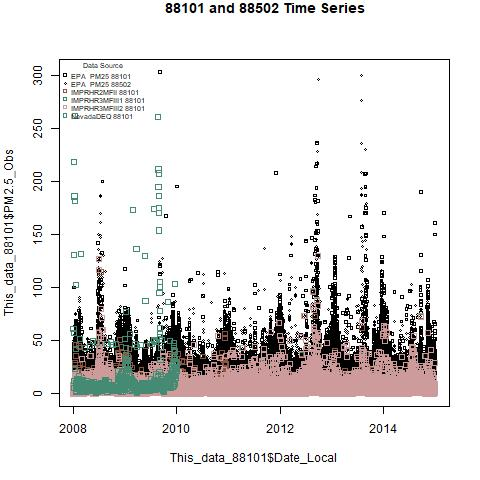
\includegraphics[width=0.77\textwidth]{Code_Outputs/TimeSeries_88101v88502.jpg} 
\caption{\label{fig:TS101v502}Time series of 88101 and 88502 PM2.5 data.} 
\end{figure} 
 
 % created from R code, not to be edited directly

%%%%%%%%%%%%%% Machine Learning %%%%%%%%%%%%%%%%%%%%

\section{Machine Learning Methods}

setting aside a portion of the PM2.5 data set and then doing 10-fold cross validation on the rest of the data

see \url{http://www.cvent.com/events/nasa-aist-machine-learning-workshop/event-summary-1f5144a5d1734ca39485d999bcdfc54a.aspx} and particularly the very end of \url{https://global.gotomeeting.com/public/recording-player.html?id=owZDmUustOjaW9sJGQ5u9cUG2pBa4D} for list of resources and papers to read.

\section{Machine Learning Results}

%[Currently, results below are derived from the example data/code from Colleen.]

%% results

\subsection{ML Inputs Time Series Images} 
 

\begin{figure} 
\centering  
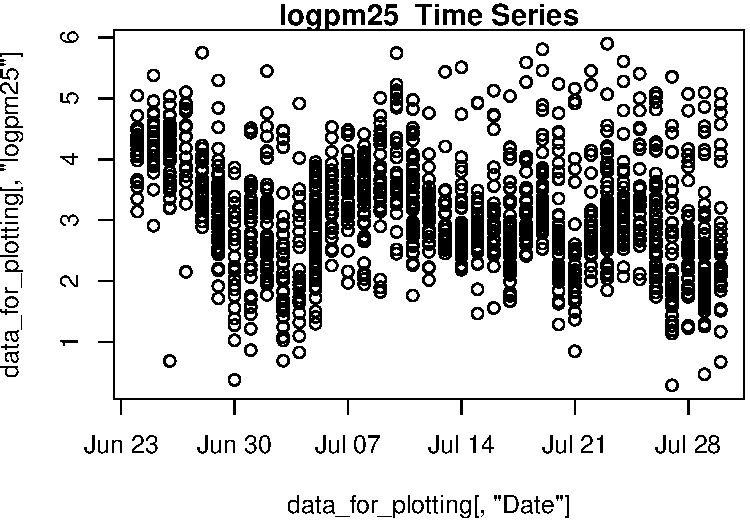
\includegraphics[width=0.77\textwidth]{Code_Outputs/ML_input_report_AllforCaret_cleaned_StepPractice_part_practice_logpm25TS.pdf} 
\caption{\label{fig:ML_input_report_AllforCaret_cleaned_StepPractice_part_practicelogpm25TS}logpm25 ML Inputs Time Series} 
\end{figure} 
 

\begin{figure} 
\centering  
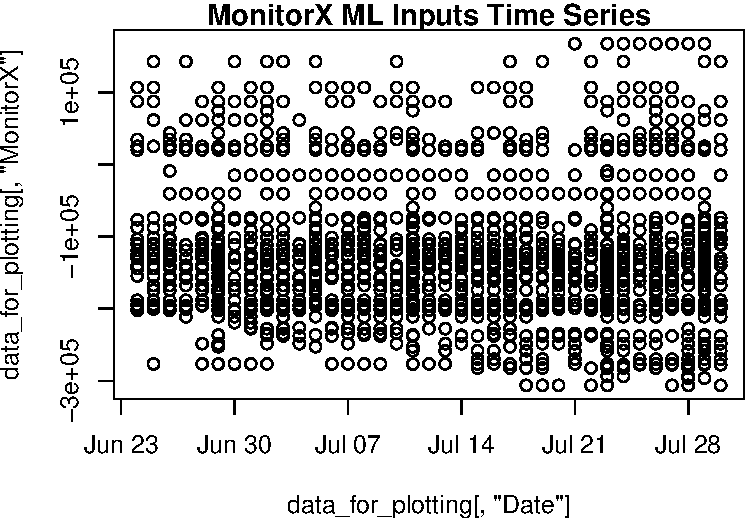
\includegraphics[width=0.77\textwidth]{Code_Outputs/ML_input_report_AllforCaret_cleaned_StepPractice_part_practice_MonitorXTS.pdf} 
\caption{\label{fig:ML_input_report_AllforCaret_cleaned_StepPractice_part_practiceMonitorXTS}MonitorX ML Inputs Time Series} 
\end{figure} 
 

\begin{figure} 
\centering  
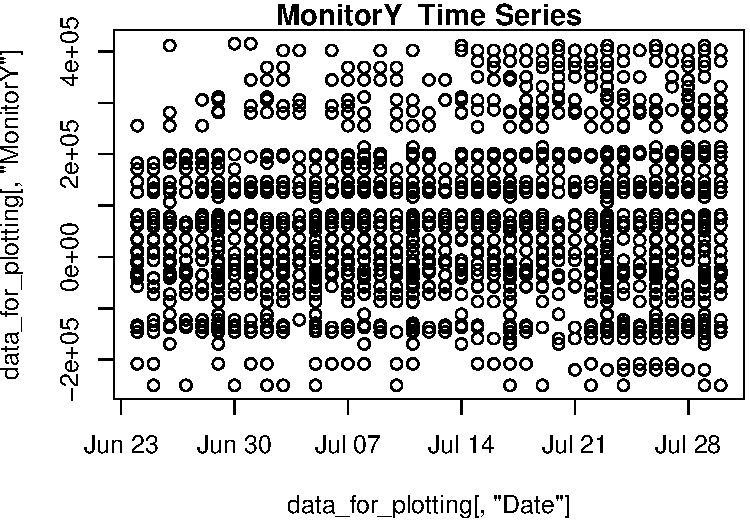
\includegraphics[width=0.77\textwidth]{Code_Outputs/ML_input_report_AllforCaret_cleaned_StepPractice_part_practice_MonitorYTS.pdf} 
\caption{\label{fig:ML_input_report_AllforCaret_cleaned_StepPractice_part_practiceMonitorYTS}MonitorY ML Inputs Time Series} 
\end{figure} 
 

\begin{figure} 
\centering  
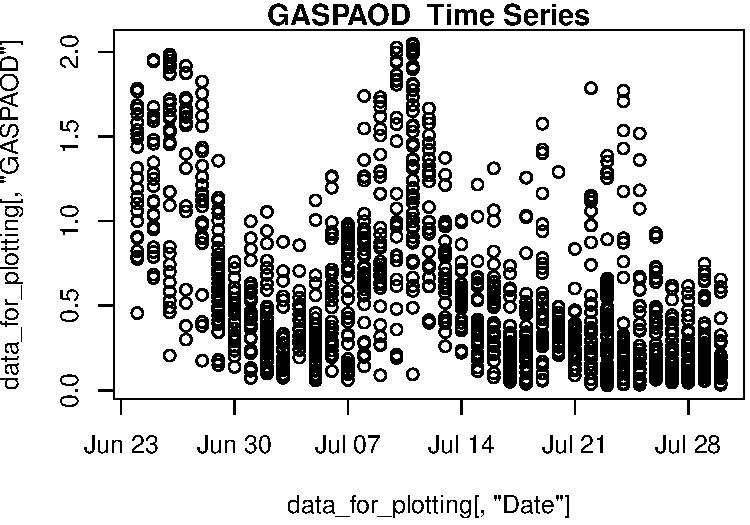
\includegraphics[width=0.77\textwidth]{Code_Outputs/ML_input_report_AllforCaret_cleaned_StepPractice_part_practice_GASPAODTS.pdf} 
\caption{\label{fig:ML_input_report_AllforCaret_cleaned_StepPractice_part_practiceGASPAODTS}GASPAOD ML Inputs Time Series} 
\end{figure} 
 

\begin{figure} 
\centering  
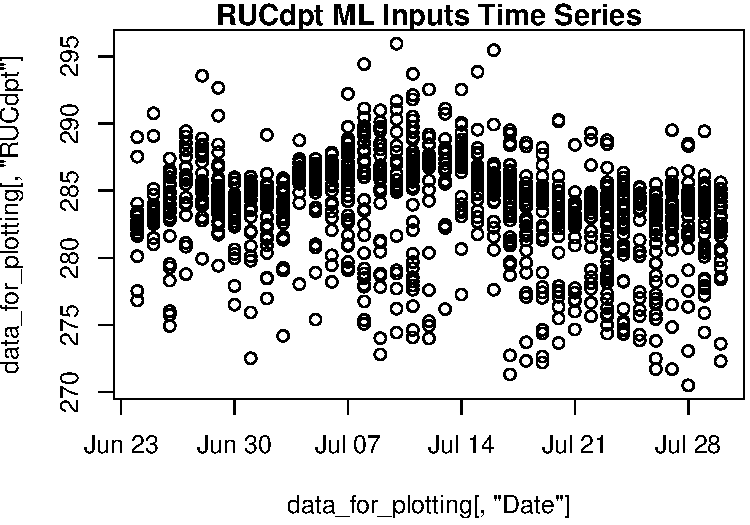
\includegraphics[width=0.77\textwidth]{Code_Outputs/ML_input_report_AllforCaret_cleaned_StepPractice_part_practice_RUCdptTS.pdf} 
\caption{\label{fig:ML_input_report_AllforCaret_cleaned_StepPractice_part_practiceRUCdptTS}RUCdpt ML Inputs Time Series} 
\end{figure} 
 

\begin{figure} 
\centering  
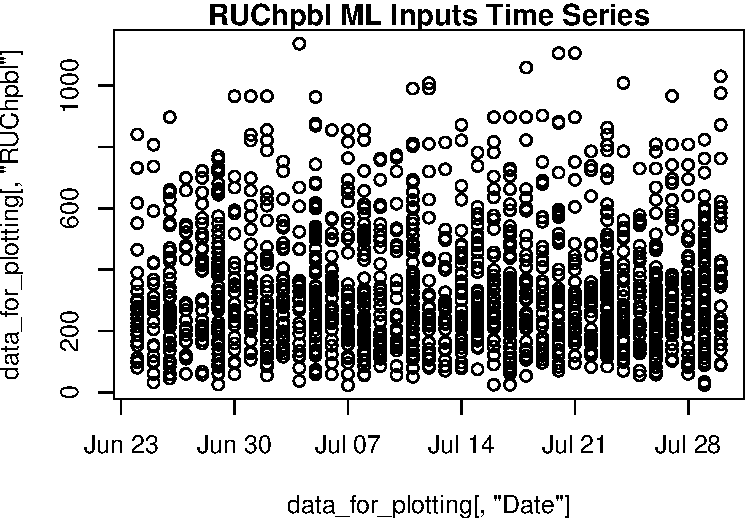
\includegraphics[width=0.77\textwidth]{Code_Outputs/ML_input_report_AllforCaret_cleaned_StepPractice_part_practice_RUChpblTS.pdf} 
\caption{\label{fig:ML_input_report_AllforCaret_cleaned_StepPractice_part_practiceRUChpblTS}RUChpbl ML Inputs Time Series} 
\end{figure} 
 

\begin{figure} 
\centering  
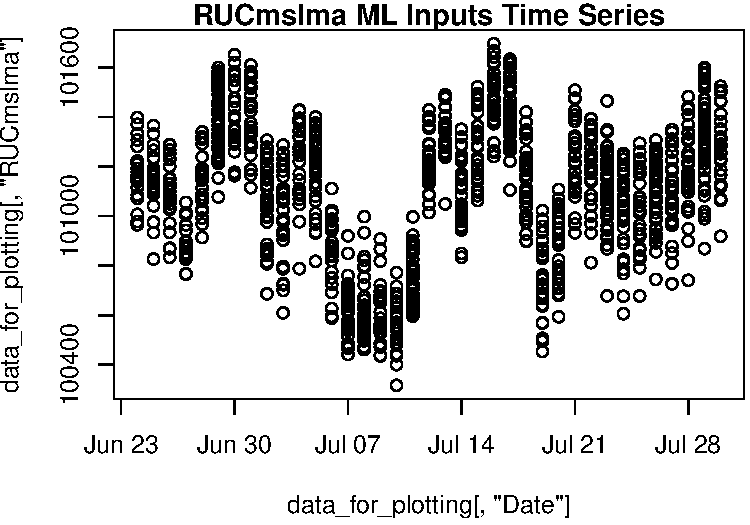
\includegraphics[width=0.77\textwidth]{Code_Outputs/ML_input_report_AllforCaret_cleaned_StepPractice_part_practice_RUCmslmaTS.pdf} 
\caption{\label{fig:ML_input_report_AllforCaret_cleaned_StepPractice_part_practiceRUCmslmaTS}RUCmslma ML Inputs Time Series} 
\end{figure} 
 

\begin{figure} 
\centering  
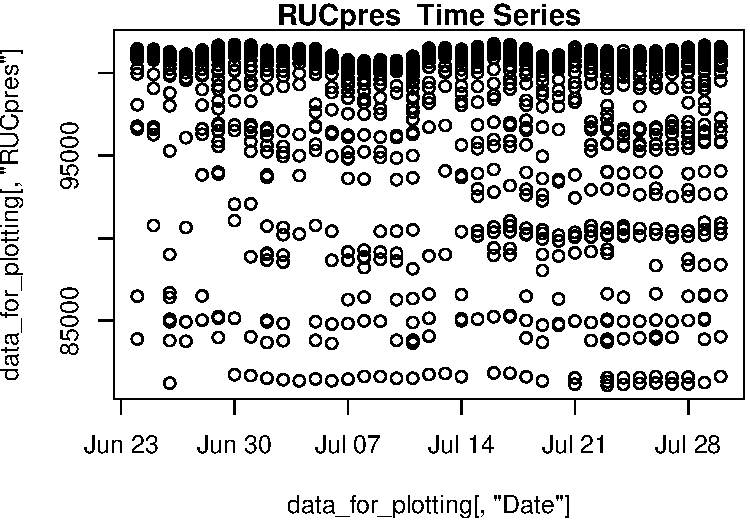
\includegraphics[width=0.77\textwidth]{Code_Outputs/ML_input_report_AllforCaret_cleaned_StepPractice_part_practice_RUCpresTS.pdf} 
\caption{\label{fig:ML_input_report_AllforCaret_cleaned_StepPractice_part_practiceRUCpresTS}RUCpres ML Inputs Time Series} 
\end{figure} 
 

\begin{figure} 
\centering  
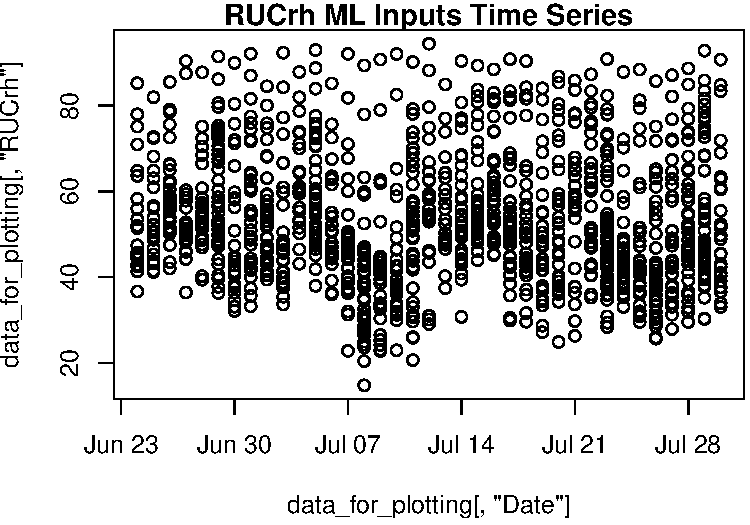
\includegraphics[width=0.77\textwidth]{Code_Outputs/ML_input_report_AllforCaret_cleaned_StepPractice_part_practice_RUCrhTS.pdf} 
\caption{\label{fig:ML_input_report_AllforCaret_cleaned_StepPractice_part_practiceRUCrhTS}RUCrh ML Inputs Time Series} 
\end{figure} 
 

\begin{figure} 
\centering  
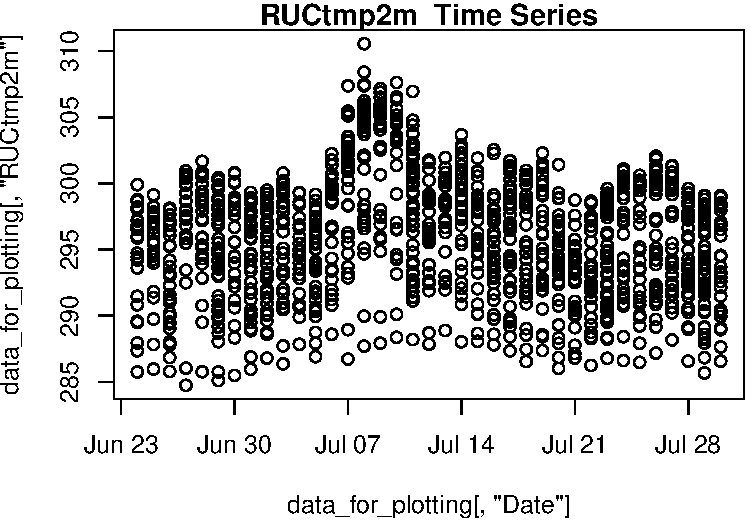
\includegraphics[width=0.77\textwidth]{Code_Outputs/ML_input_report_AllforCaret_cleaned_StepPractice_part_practice_RUCtmp2mTS.pdf} 
\caption{\label{fig:ML_input_report_AllforCaret_cleaned_StepPractice_part_practiceRUCtmp2mTS}RUCtmp2m ML Inputs Time Series} 
\end{figure} 
 

\begin{figure} 
\centering  
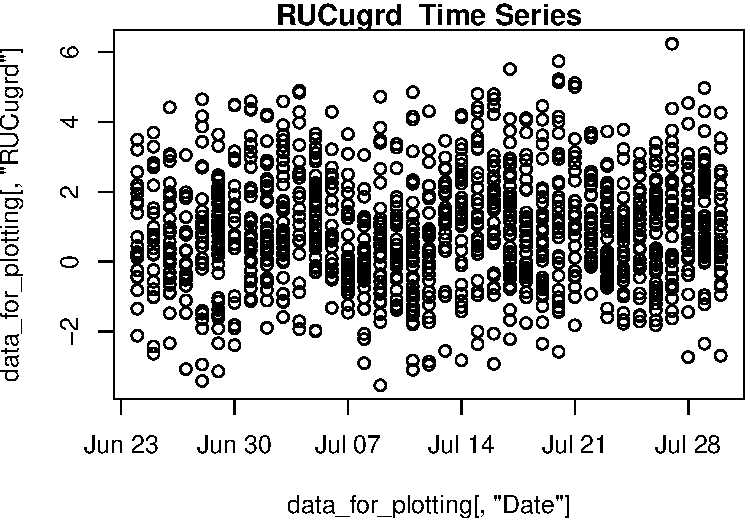
\includegraphics[width=0.77\textwidth]{Code_Outputs/ML_input_report_AllforCaret_cleaned_StepPractice_part_practice_RUCugrdTS.pdf} 
\caption{\label{fig:ML_input_report_AllforCaret_cleaned_StepPractice_part_practiceRUCugrdTS}RUCugrd ML Inputs Time Series} 
\end{figure} 
 

\begin{figure} 
\centering  
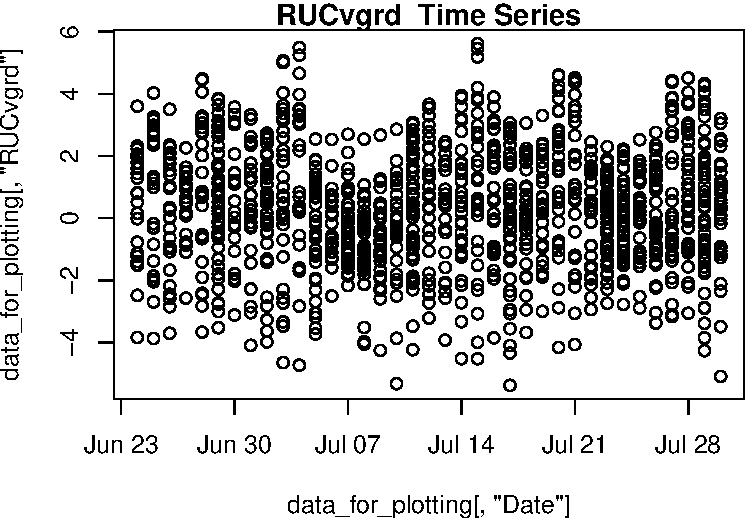
\includegraphics[width=0.77\textwidth]{Code_Outputs/ML_input_report_AllforCaret_cleaned_StepPractice_part_practice_RUCvgrdTS.pdf} 
\caption{\label{fig:ML_input_report_AllforCaret_cleaned_StepPractice_part_practiceRUCvgrdTS}RUCvgrd ML Inputs Time Series} 
\end{figure} 
 

\begin{figure} 
\centering  
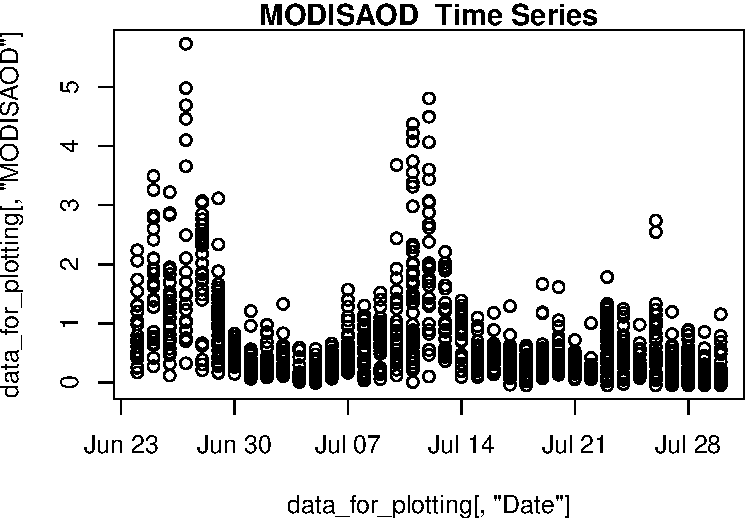
\includegraphics[width=0.77\textwidth]{Code_Outputs/ML_input_report_AllforCaret_cleaned_StepPractice_part_practice_MODISAODTS.pdf} 
\caption{\label{fig:ML_input_report_AllforCaret_cleaned_StepPractice_part_practiceMODISAODTS}MODISAOD ML Inputs Time Series} 
\end{figure} 
 

\begin{figure} 
\centering  
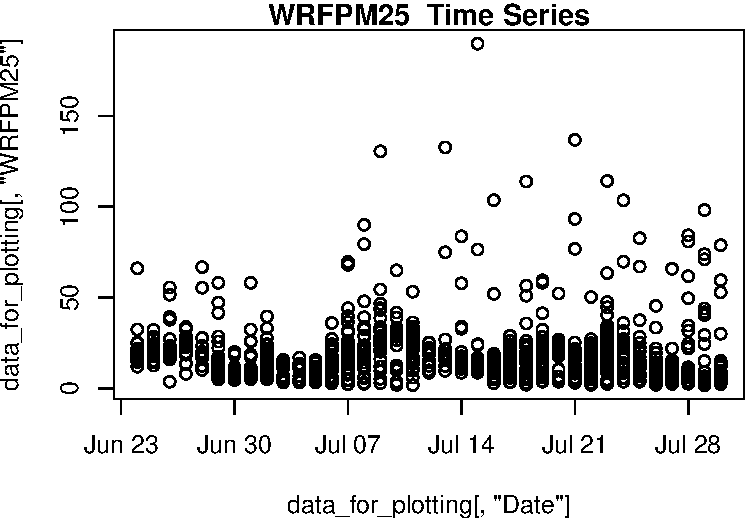
\includegraphics[width=0.77\textwidth]{Code_Outputs/ML_input_report_AllforCaret_cleaned_StepPractice_part_practice_WRFPM25TS.pdf} 
\caption{\label{fig:ML_input_report_AllforCaret_cleaned_StepPractice_part_practiceWRFPM25TS}WRFPM25 ML Inputs Time Series} 
\end{figure} 
 

\begin{figure} 
\centering  
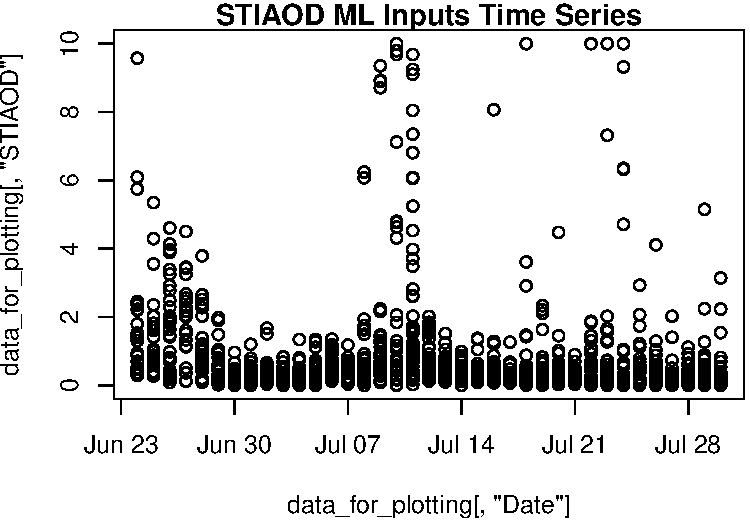
\includegraphics[width=0.77\textwidth]{Code_Outputs/ML_input_report_AllforCaret_cleaned_StepPractice_part_practice_STIAODTS.pdf} 
\caption{\label{fig:ML_input_report_AllforCaret_cleaned_StepPractice_part_practiceSTIAODTS}STIAOD ML Inputs Time Series} 
\end{figure} 
 

\begin{figure} 
\centering  
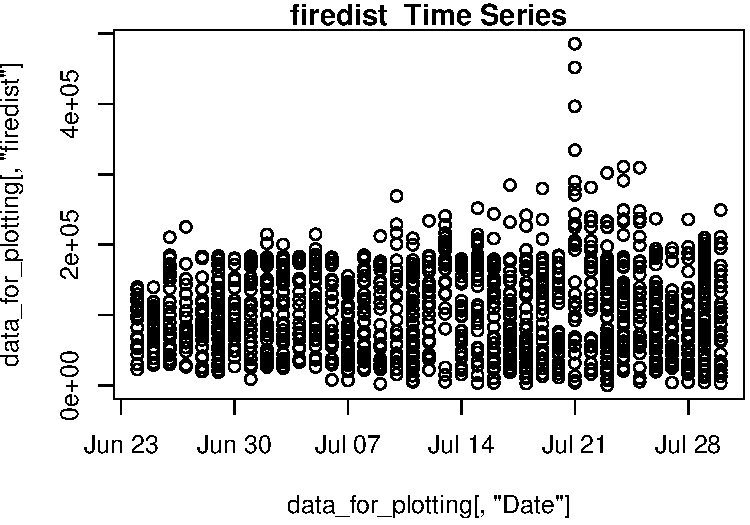
\includegraphics[width=0.77\textwidth]{Code_Outputs/ML_input_report_AllforCaret_cleaned_StepPractice_part_practice_firedistTS.pdf} 
\caption{\label{fig:ML_input_report_AllforCaret_cleaned_StepPractice_part_practicefiredistTS}firedist ML Inputs Time Series} 
\end{figure} 
 

\begin{figure} 
\centering  
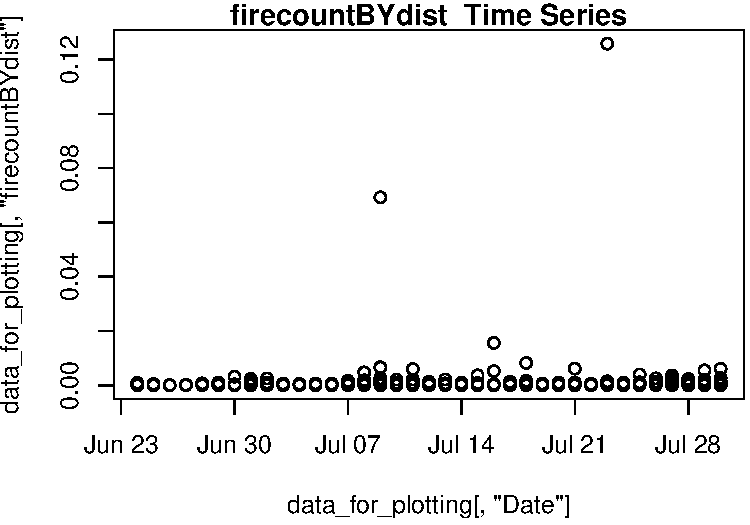
\includegraphics[width=0.77\textwidth]{Code_Outputs/ML_input_report_AllforCaret_cleaned_StepPractice_part_practice_firecountBYdistTS.pdf} 
\caption{\label{fig:ML_input_report_AllforCaret_cleaned_StepPractice_part_practicefirecountBYdistTS}firecountBYdist ML Inputs Time Series} 
\end{figure} 
 

\begin{figure} 
\centering  
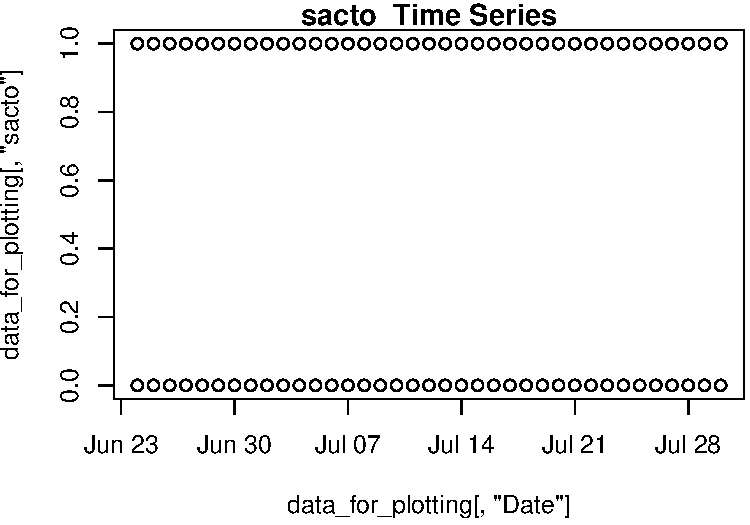
\includegraphics[width=0.77\textwidth]{Code_Outputs/ML_input_report_AllforCaret_cleaned_StepPractice_part_practice_sactoTS.pdf} 
\caption{\label{fig:ML_input_report_AllforCaret_cleaned_StepPractice_part_practicesactoTS}sacto ML Inputs Time Series} 
\end{figure} 
 

\begin{figure} 
\centering  
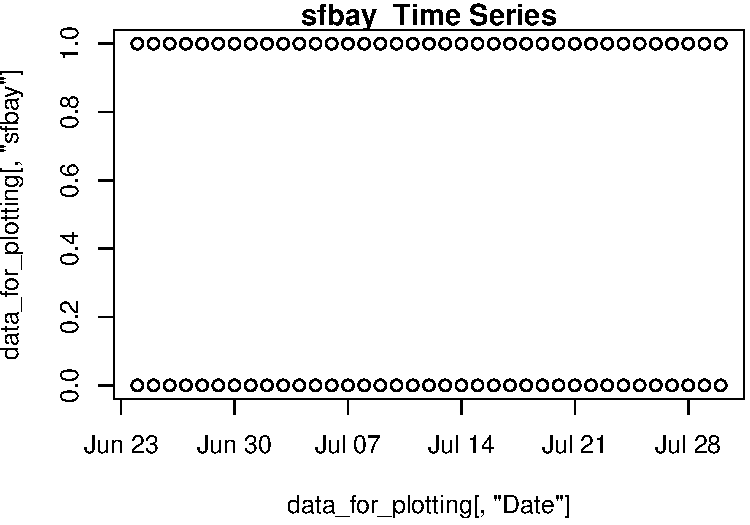
\includegraphics[width=0.77\textwidth]{Code_Outputs/ML_input_report_AllforCaret_cleaned_StepPractice_part_practice_sfbayTS.pdf} 
\caption{\label{fig:ML_input_report_AllforCaret_cleaned_StepPractice_part_practicesfbayTS}sfbay ML Inputs Time Series} 
\end{figure} 
 

\begin{figure} 
\centering  
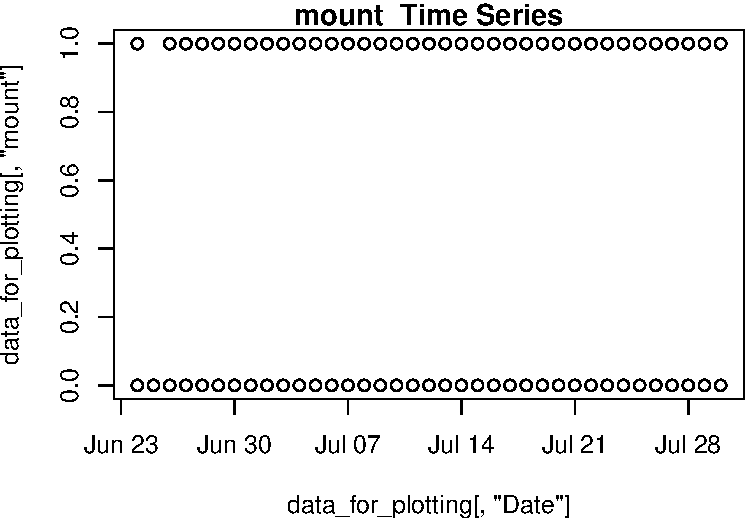
\includegraphics[width=0.77\textwidth]{Code_Outputs/ML_input_report_AllforCaret_cleaned_StepPractice_part_practice_mountTS.pdf} 
\caption{\label{fig:ML_input_report_AllforCaret_cleaned_StepPractice_part_practicemountTS}mount ML Inputs Time Series} 
\end{figure} 
 

\begin{figure} 
\centering  
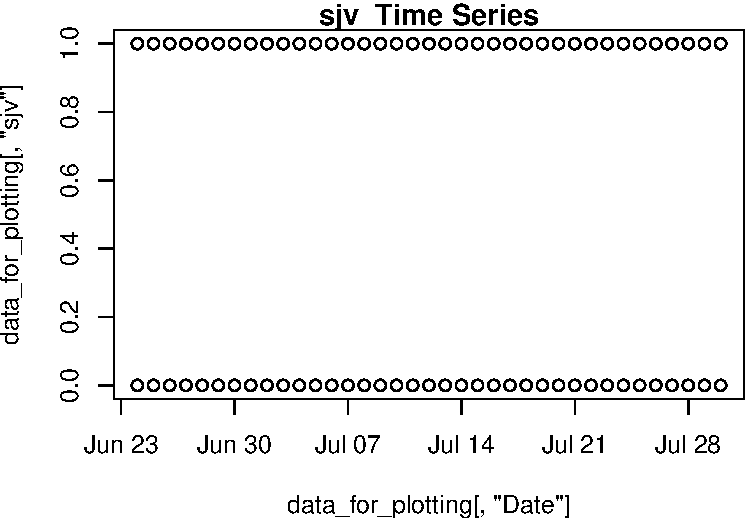
\includegraphics[width=0.77\textwidth]{Code_Outputs/ML_input_report_AllforCaret_cleaned_StepPractice_part_practice_sjvTS.pdf} 
\caption{\label{fig:ML_input_report_AllforCaret_cleaned_StepPractice_part_practicesjvTS}sjv ML Inputs Time Series} 
\end{figure} 
 

\begin{figure} 
\centering  
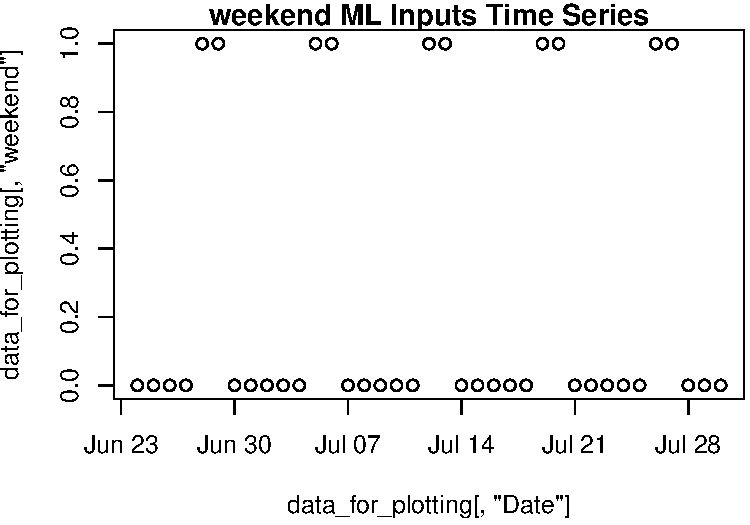
\includegraphics[width=0.77\textwidth]{Code_Outputs/ML_input_report_AllforCaret_cleaned_StepPractice_part_practice_weekendTS.pdf} 
\caption{\label{fig:ML_input_report_AllforCaret_cleaned_StepPractice_part_practiceweekendTS}weekend ML Inputs Time Series} 
\end{figure} 
 

\begin{figure} 
\centering  
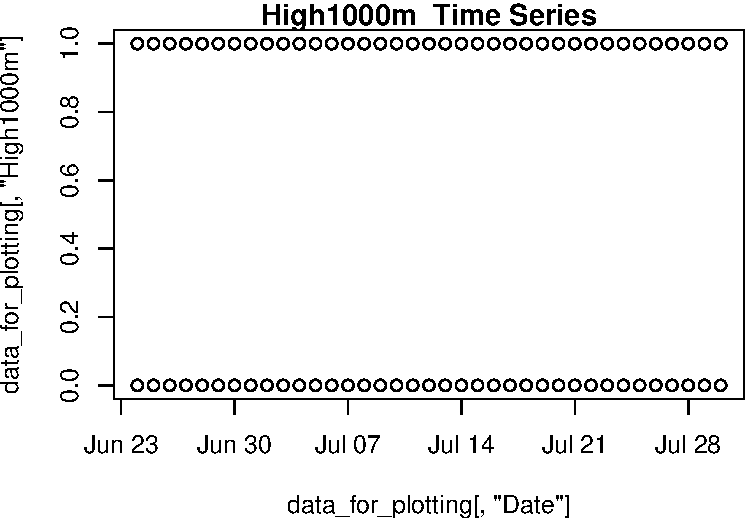
\includegraphics[width=0.77\textwidth]{Code_Outputs/ML_input_report_AllforCaret_cleaned_StepPractice_part_practice_High1000mTS.pdf} 
\caption{\label{fig:ML_input_report_AllforCaret_cleaned_StepPractice_part_practiceHigh1000mTS}High1000m ML Inputs Time Series} 
\end{figure} 
 

\begin{figure} 
\centering  
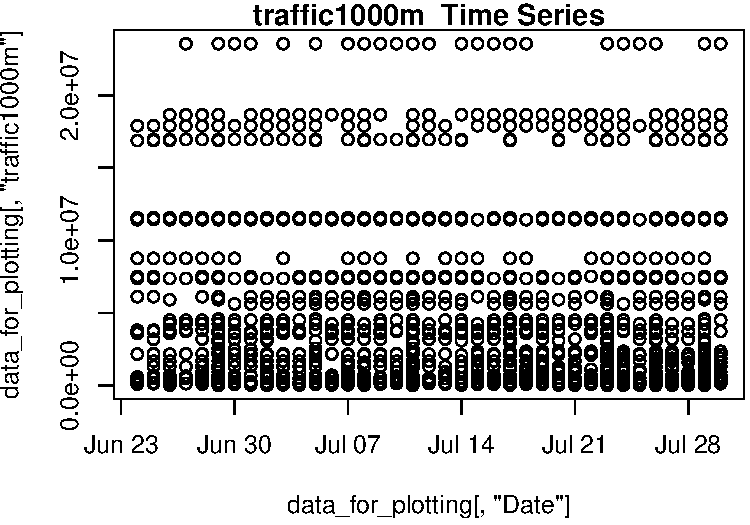
\includegraphics[width=0.77\textwidth]{Code_Outputs/ML_input_report_AllforCaret_cleaned_StepPractice_part_practice_traffic1000mTS.pdf} 
\caption{\label{fig:ML_input_report_AllforCaret_cleaned_StepPractice_part_practicetraffic1000mTS}traffic1000m ML Inputs Time Series} 
\end{figure} 
 

\begin{figure} 
\centering  
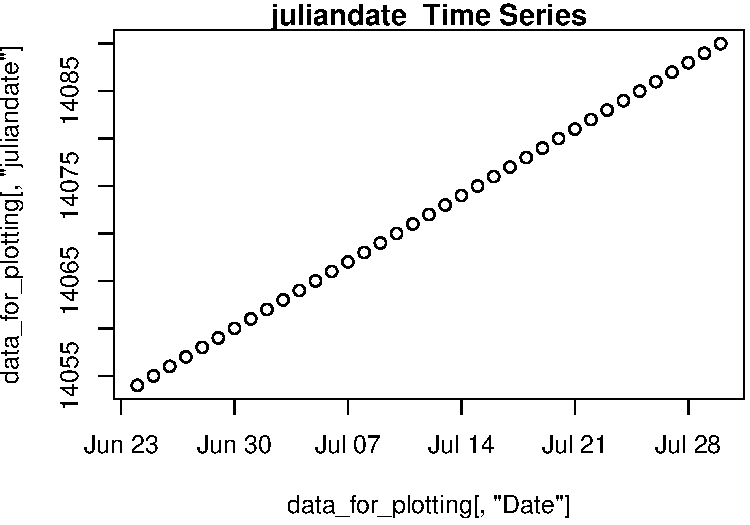
\includegraphics[width=0.77\textwidth]{Code_Outputs/ML_input_report_AllforCaret_cleaned_StepPractice_part_practice_juliandateTS.pdf} 
\caption{\label{fig:ML_input_report_AllforCaret_cleaned_StepPractice_part_practicejuliandateTS}juliandate ML Inputs Time Series} 
\end{figure} 
 

\begin{figure} 
\centering  
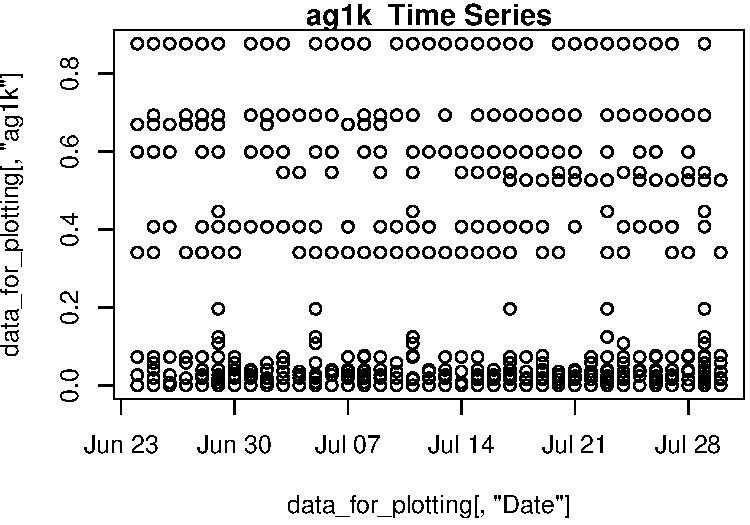
\includegraphics[width=0.77\textwidth]{Code_Outputs/ML_input_report_AllforCaret_cleaned_StepPractice_part_practice_ag1kTS.pdf} 
\caption{\label{fig:ML_input_report_AllforCaret_cleaned_StepPractice_part_practiceag1kTS}ag1k ML Inputs Time Series} 
\end{figure} 
 

\begin{figure} 
\centering  
\includegraphics[width=0.77\textwidth]{Code_Outputs/ML_input_report_AllforCaret_cleaned_StepPractice_part_practice_urban1kTS.pdf} 
\caption{\label{fig:ML_input_report_AllforCaret_cleaned_StepPractice_part_practiceurban1kTS}urban1k ML Inputs Time Series} 
\end{figure} 
 

\begin{figure} 
\centering  
\includegraphics[width=0.77\textwidth]{Code_Outputs/ML_input_report_AllforCaret_cleaned_StepPractice_part_practice_veg1kTS.pdf} 
\caption{\label{fig:ML_input_report_AllforCaret_cleaned_StepPractice_part_practiceveg1kTS}veg1k ML Inputs Time Series} 
\end{figure} 
 

\begin{figure} 
\centering  
\includegraphics[width=0.77\textwidth]{Code_Outputs/ML_input_report_AllforCaret_cleaned_StepPractice_part_practice_elevationTS.pdf} 
\caption{\label{fig:ML_input_report_AllforCaret_cleaned_StepPractice_part_practiceelevationTS}elevation ML Inputs Time Series} 
\end{figure} 
 

\begin{figure} 
\centering  
\includegraphics[width=0.77\textwidth]{Code_Outputs/ML_input_report_AllforCaret_cleaned_StepPractice_part_practice_PopDenTS.pdf} 
\caption{\label{fig:ML_input_report_AllforCaret_cleaned_StepPractice_part_practicePopDenTS}PopDen ML Inputs Time Series} 
\end{figure} 
 

\clearpage

\subsection{ranger 1 Images} 
 

\begin{figure} 
\centering  
\includegraphics[width=0.77\textwidth]{Code_Outputs/ML_report_task_1ranger_RMSEvNVariables.pdf} 
\caption{\label{fig:ML_report_task_1rangerRMSEvNVariables}ranger 1.} 
\end{figure} 
 
 % created from R code, not to be edited directly
\clearpage

\subsection{glmnet 2 Images} 
 

\begin{figure} 
\centering  
\includegraphics[width=0.77\textwidth]{Code_Outputs/ML_report_task_2glmnet_RMSEvNVariables.pdf} 
\caption{\label{fig:ML_report_task_2glmnetRMSEvNVariables}glmnet 2.} 
\end{figure} 
 
 % created from R code, not to be edited directly
\clearpage

\subsection{Compare multiple models Images} 
 

\begin{figure} 
\centering  
\includegraphics[width=0.77\textwidth]{Code_Outputs/ML_compare_models_bwplot_all.pdf} 
\caption{\label{fig:ML_compare_modelsbwplot_all}Box and whisker plots for all metrics together..} 
\end{figure} 
 

\begin{figure} 
\centering  
\includegraphics[width=0.77\textwidth]{Code_Outputs/ML_compare_models_bwplot_RMSE.pdf} 
\caption{\label{fig:ML_compare_modelsbwplot_RMSE}Box and whisker plots for RMSE.} 
\end{figure} 
 

\begin{figure} 
\centering  
\includegraphics[width=0.77\textwidth]{Code_Outputs/ML_compare_models_bwplot_Rsquared.pdf} 
\caption{\label{fig:ML_compare_modelsbwplot_Rsquared}Box and whisker plots for Rsquared.} 
\end{figure} 
 

\begin{figure} 
\centering  
\includegraphics[width=0.77\textwidth]{Code_Outputs/ML_compare_models_bwplot_MAE.pdf} 
\caption{\label{fig:ML_compare_modelsbwplot_MAE}Box and whisker plots for MAE.} 
\end{figure} 
 

\begin{figure} 
\centering  
\includegraphics[width=0.77\textwidth]{Code_Outputs/ML_compare_models_dotplot_RMSE.pdf} 
\caption{\label{fig:ML_compare_modelsdotplot_RMSE}Dot plots for RMSE.} 
\end{figure} 
 

\begin{figure} 
\centering  
\includegraphics[width=0.77\textwidth]{Code_Outputs/ML_compare_models_dotplot_Rsquared.pdf} 
\caption{\label{fig:ML_compare_modelsdotplot_Rsquared}Dot plots for Rsquared.} 
\end{figure} 
 

\begin{figure} 
\centering  
\includegraphics[width=0.77\textwidth]{Code_Outputs/ML_compare_models_dotplot_MAE.pdf} 
\caption{\label{fig:ML_compare_modelsdotplot_MAE}Dot plots for MAE.} 
\end{figure} 
 

\begin{figure} 
\centering  
\includegraphics[width=0.77\textwidth]{Code_Outputs/ML_compare_models_densityplot_RMSE.pdf} 
\caption{\label{fig:ML_compare_modelsdensityplot_RMSE}Density plots for RMSE.} 
\end{figure} 
 

\begin{figure} 
\centering  
\includegraphics[width=0.77\textwidth]{Code_Outputs/ML_compare_models_densityplot_Rsquared.pdf} 
\caption{\label{fig:ML_compare_modelsdensityplot_Rsquared}Density plots for Rsquared.} 
\end{figure} 
 

\begin{figure} 
\centering  
\includegraphics[width=0.77\textwidth]{Code_Outputs/ML_compare_models_densityplot_MAE.pdf} 
\caption{\label{fig:ML_compare_modelsdensityplot_MAE}Density plots for MAE.} 
\end{figure} 
 

\begin{figure} 
\centering  
\includegraphics[width=0.77\textwidth]{Code_Outputs/ML_compare_models_xyplot_RMSE.pdf} 
\caption{\label{fig:ML_compare_modelsxyplot_RMSE}Scatter plot for RMSE.} 
\end{figure} 
 

\begin{figure} 
\centering  
\includegraphics[width=0.77\textwidth]{Code_Outputs/ML_compare_models_xyplot_Rsquared.pdf} 
\caption{\label{fig:ML_compare_modelsxyplot_Rsquared}Scatter plot for Rsquared.} 
\end{figure} 
 

\begin{figure} 
\centering  
\includegraphics[width=0.77\textwidth]{Code_Outputs/ML_compare_models_xyplot_MAE.pdf} 
\caption{\label{fig:ML_compare_modelsxyplot_MAE}Scatter plot for MAE.} 
\end{figure} 
 

\clearpage

\subsection{Geometric Centroids of Counties Images} 
 

\begin{figure} 
\centering  
\includegraphics[width=0.77\textwidth]{Code_Outputs/CountyGeometricCentroids_MapLocations.jpg} 
\caption{\label{fig:CountyGeometricCentroidsMapLocations}Geometric Centroids of Counties} 
\end{figure} 
 

%\include{RF1Images}

%\include{Treebag1Images}

%\include{GBMImages}

%\include{Data_Processing}

%%%% Bibliography %%%%
\clearpage
\addcontentsline{toc}{section}{References} % make References show up in table of contents
\bibliographystyle{apalike}%{plainnat}%{vancouver}%{alpha}
\bibliography{ReidGroupReferences}

%%%% Supplemental Material %%%%

% figures of every numerical column in PM2.5 data



%%%% KEEP example commenting code %%%%
%Comments can also be added to the margins of the compiled PDF using the todo command\todo{Here's a comment in the margin!}, as shown in the example on the right. You can also add inline comments:

%\todo[inline, color=green!40]{This is an inline comment.}
%%%%%%%%

\end{document}
